\chapter{Rating by ranking with learned performance quantile norms}
\label{sec:10}

\abstract*{ We address in Chapter~\ref{sec:10} the problem of rating multiple criteria performances of a set of potential decision alternatives with respect to performance quantiles learned from historical performance data gathered from similar decision alternatives observed in the past. We show how to learn performance quantiles from historical performance tableaux. New performance records may now be rated with respect to these quantile norms.}

\abstract{ We address in Chapter~\ref{sec:10} the problem of rating multiple criteria performances of a set of potential decision alternatives with respect to performance quantiles learned from historical performance data gathered from similar decision alternatives observed in the past. We show how to learn performance quantiles from historical performance tableaux. New performance records may now be rated with respect to these quantile norms.}

\section{The absolute rating problem}
\label{sec:10.1}
	  
To illustrate the \emph{absolute rating} problem we face, consider for a moment that, in a given decision making problem, we observe, for instance, in Table \ref{tab:10.1} below, the multi-criteria performances of two potential decision alternatives, named \texttt{a1001} and \texttt{a1010}, graded on 7 \emph{incommensurable} preformance criteria: 2 \emph{Costs} criteria \texttt{c1} and \texttt{c2} (to \emph{minimize}) and 5 \emph{Benefits} criteria \texttt{b1} to \texttt{b5} (to \emph{maximize}). 
\begin{table}[h]
\caption{Multi-criteria performances of two potential decision alternatives}
\label{tab:10.1}       % Give a unique label
\begin{center}
  %\begin{small}
    \begin{tabular}{l|c|c|c|c|c|c|c}
      \svhline\noalign{\smallskip}
      Criterion (weight) & \texttt{b1} (2) & \texttt{b2} (2) & \texttt{b3} (2) & \texttt{b4} (2) & \texttt{b5} (2) & \texttt{c1} (5) & \texttt{c2} (5)\\
      \noalign{\smallskip}\hline\noalign{\smallskip}
    \texttt{a1001} &   37.0  &  2 & 2 & 61.0 & 31.0 & -4 & -40.0\\
    \texttt{a1010} &   32.0 & 9 & 6 & 55.0 & 51.0 & -4 & -35.0 \\
      \noalign{\smallskip}\hline
    \end{tabular}
  %\end{small}
\end{center}
\end{table}
The performances on \emph{Benefits} criteria \texttt{b1}, \texttt{b4} and \texttt{b5} are measured on a cardinal scale from $0.0$ (worst) to $100.0$ (best) whereas, the performances on the \emph{Benefits} criteria \texttt{b2} and \texttt{b3}  and on the \emph{Costs} criterion \texttt{c1} are measured on an ordinal scale from $0$ (worst) to $10$ (best), respectively $-10$ (worst) to $0$ (best). The performances on the \emph{Costs} criterion \texttt{c2} are eventually measured on a cardinal \emph{negative} scale from $-100.00$ (worst) to $0.0$ (best). The two \emph{Costs} criteria are equi-significant (weight 5). Similarly, the five Benefits criteria are also equi-significant (weight 2). The \emph{importance} (sum of significance weights: $2 \times 5 = 10$) of the \emph{Costs} criteria is hence \emph{equivalent} to the \emph{importance} (sum of significance weights: $5 \times 2 = 10$) of the \emph{Benefits} criteria.
   
The non trivial decision problem we now face here, is to decide, how the previous two multiple criteria performances of \texttt{a1001}, respectively \texttt{a1010},  may be rated (\emph{excellent}~? \emph{good}~?, or \emph{fair}~?; perhaps even, \emph{weak}~? or \emph{very weak}~?) in an \emph{order statistical sense}, when compared with similar multi-criteria performances one has already encountered in the past. 

To solve this \emph{absolute} rating problem, first, we need to estimate multi-criteria \emph{performance quantiles} from historical records\footnote{See Lecture 5 of the Computational Statistics Course \citep{CPSTAT-L5}.}.  

\section{Incremental learning of historical performance quantiles}
\label{sec:10.2}

Suppose that we see flying in random multiple criteria performances from a given model of random performance tableau (see Chapter \ref{sec:5}). The question we address here is to estimate empirical performance quantiles on the basis of so far observed performance vectors. For this task, we are inspired by \citep*{CHAM-2006}, who present an efficient algorithm for incrementally updating a quantile-binned cumulative distribution function (CDF) with newly observed CDFs\footnote{We have adapted a C++ implementation published by \citep*[Chapter 5]{NR3-2007}.}. 

The \texttt{PerformanceQuantiles}\index{PerformanceQuantiles@\texttt{PerformanceQuantiles} class} class, using the\\ \texttt{IncrementalQuantilesEstimator} class\index{IncrementalQuantilesEstimator@\texttt{IncrementalQuantilesEstimator} class} from the \texttt{randomNumbers} module \index{randomNumbers@\texttt{randomNumbers} module}, implements such a performance quantiles estimation based on a given performance tableau. Its main attributes are:
\begin{itemize}[rightmargin=0.5cm,leftmargin=0.5cm]
\item Ordered \texttt{objectives} and a \texttt{criteria} dictionaries from a valid performance tableau instance;
\item A list \texttt{quantileFrequencies} of quantile frequencies like:
  \begin{itemize}[nosep]
  \item \emph{quartiles} $[0.0, 0.25, 05, 0.75,1.0]$,
  \item  \emph{quintiles} $[0.0, 0.2, 0.4, 0.6, 0.8, 1.0]$ or
  \item  \emph{deciles} $[0.0, 0.1, 0.2, ... 1.0]$ for instance;
  \end{itemize}
\item An ordered  dictionary \texttt{limitingQuantiles} of so far estimated \emph{lower} (default) or \emph{upper} quantile class limits for each frequency per criterion;
\item An ordered dictionary \texttt{historySizes} for keeping track of the number of evaluations seen so far per criterion. Missing data, the case given, make these sizes vary from criterion to criterion.
\end{itemize}

Below, we show an example Python session concerning 900 decision alternatives randomly generated with a \emph{Cost-Benefit} performance tableau model (see Section \ref{sec:5.3}) from which are also drawn the performances of alternatives \texttt{a1001} and \texttt{a1010} shown in Table \ref{tab:10.1} above.
\begin{lstlisting}[caption={Computing performance quantiles from a given performance tableau},label=list:10.1]
>>> from performanceQuantiles import PerformanceQuantiles
>>> from randomPerfTabs import RandomCBPerformanceTableau
>>> nbrActions=900
>>> nbrCrit = 7
>>> seed = 100
>>> pt = RandomCBPerformanceTableau(numberOfActions=nbrActions,\
...                  numberOfCriteria=nbrCrit,seed=seed)
>>> pq = PerformanceQuantiles(pt,\
...                   numberOfBins = 'quartiles',\
...                   LowerClosed=True)
>>> pq
  *------- PerformanceQuantiles instance description ------*
   Instance class   : PerformanceQuantiles
   Instance name    : 4-tiled_performances
   Objectives       : 2
   Criteria         : 7
   Quantiles        : 4
   History sizes    : {'c1': 887,'b1': 888,'b2': 891,'b3': 895,
                        'b4': 892,'c2': 893,'b5': 887}
   Attributes       : ['perfTabType','valueDigits',
                       'actionsTypeStatistics',
                       'objectives', 'BigData',
                       'missingDataProbability',
		       'criteria', 'LowerClosed', 'name',
		       'quantilesFrequencies', 'historySizes',
		       'limitingQuantiles', 'cdf']
\end{lstlisting}
The \texttt{PerformanceQuantiles} class parameter \texttt{numberOfBins} (see Listing \ref{list:10.1} Line 9 above), choosing the wished number of quantile frequencies, may be either \emph{quartiles} (4 bins), \emph{quintiles} (5 bins), \emph{deciles} (10 bins), \emph{dodeciles} (20 bins) or any other integer number of quantile bins. The quantile bins may be either \emph{lower closed} (default) or \emph{upper-closed}.

Inspecting the estimated quartile limits may be operated with the\\ \texttt{showLimitingQuantiles()} method.\index{showLimitingQuantiles@\texttt{showLimitingQuantiles()}}
\begin{lstlisting}[caption={Printing out the estimated quartile limits},label=list:10.2]
>>> pq.showLimitingQuantiles(ByObjectives=True)
    ----  Historical performance quantiles -----*
    Costs
    criteria | weights |  '0.00' '0.25' '0.50' '0.75' '1.00'   
    ---------|----------------------------------------------------
       'c1'  |    5    |   -10    -7     -5     -3      0  
       'c2'  |    5    | -96.37 -70.65 -50.10 -30.00  -1.43  
    Benefits
    criteria | weights | '0.00'  '0.25' '0.50' '0.75' '1.00'   
    ---------|-----------------------------------------------------
       'b1'  |    2    |  1.99    29.82 49.44  70.73  99.83  
       'b2'  |    2    |    0      3      5      7     10  
       'b3'  |    2    |    0      3      5      7     10  
       'b4'  |    2    |  3.27   30.10  50.82  70.89  98.05  
       'b5'  |    2    |  0.85   29.08  48.55  69.98  97.56  
\end{lstlisting}
Both objectives are \emph{equi-important}; the sum of weights (10) of the \emph{Costs} criteria balance the sum of weights (10) of the \emph{Benefits} criteria (see Listing \ref{list:10.2} column 2). The preference direction of the \emph{Costs} criteria \texttt{c1} and \texttt{c2} is \emph{negative}; the lesser the costs, the better it is, whereas all the \emph{Benefits} criteria \texttt{b1} to \texttt{b5} show \emph{positive} preference directions, i.e. the higher the benefits, the better it is. The columns entitled '$0.00$', resp. '$1.00$' show the \emph{quartile} \texttt{Q0}, resp. \texttt{Q4}, i.e. the \emph{worst}, resp. \emph{best} performance observed so far on each criterion. Column '$0.50$' shows the \emph{median} (\texttt{Q2}) performance observed on the criteria.  

New  decision alternatives with random multiple criteria performance vectors from the same random performance tableau model as \texttt{pt} (see Listing~\ref{list:10.1}) may now be generated with a generic \texttt{RandomPerformanceGenerator} class\index{RandomPerformanceGenerator@\texttt{RandomPerformanceGenerator()}}, provided in the \texttt{randomPerfTabs} module.\footnote{The \texttt{RandomPerformanceGenerator} class works for the \emph{standard} performance tableau model (see Section \ref{sec:5.2}), the \emph{Cost-Benefit} model (see Section \ref{sec:5.3}), and the 3-objectives model (see Section \ref{sec:5.4}).}
\begin{lstlisting}[caption={Generating 100 new random decision alternatives of the same model},label=list:10.3]
>>> from randomPerfTabs import RandomPerformanceGenerator
>>> rpg = RandomPerformanceGenerator(tp,seed=seed)
>>> newTab = rpg.randomPerformanceTableau(100)
\end{lstlisting}

The so far estimated historical quantile limits may be updated with this newly arriving 100 data records:
\begin{lstlisting}
>>> # Updating the quartile norms shown above 
>>> pq.updateQuantiles(newTab,historySize=None)
\end{lstlisting}
Parameter \texttt{historySize} of the \texttt{updateQuantiles()} method (Line 2 above) allows to \emph{balance} the \emph{new} evaluations against the \emph{historical} ones.

With \texttt{historySize = None} (the default setting), the balance in the example above is $900/1000$ ($90\%$, the weight of historical data) against $100/1000$ ($10\%$, the weight of the new incoming observations). Putting \texttt{historySize = 0}, for instance, will ignore all historical data ($0/100$ against $100/100$) and restart building the quantile estimation with solely the new incoming data. The updated quantile limits may be shown in a browser view (see Fig. \ref{fig:10.1}).
\begin{lstlisting}
>>> # showing the updated quantile limits in a browser view
>>> pq.showHTMLLimitingQuantiles(Transposed=True)
\end{lstlisting}
\begin{figure}[h]
\sidecaption[t]
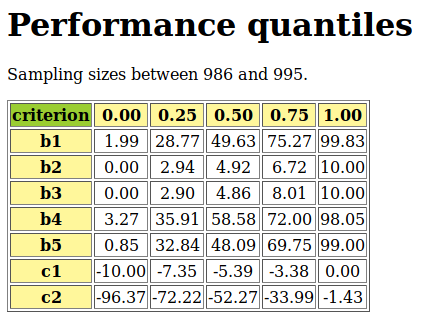
\includegraphics[width=7cm]{Figures/examplePerfQuantiles.png}
\caption{Showing updated quartiles limits per criterion. The $0.25$ column shows the first quartile (\texttt{Q1}) limits, the $0.50$ column shows the second quartile (\texttt{Q2}) limits and the $0.75$ column shows the third quartile (\texttt{Q3}) limits. Column $0.00$ (resp. $1.00$) shows the minimum (resp. maximum) performance on each criterion.}
\label{fig:10.1}       % Give a unique label
\end{figure}
    
\section{Rating-by-ranking new performances with quantile norms}
\label{sec:10.3}

For \emph{rating} a newly given set of decision alternatives with the help of empirical performance quantiles estimated from historical data, we provide the \texttt{Learned\-QuantilesRatingDigraph} class\index{LearnedQuantilesRatingDigraph@\texttt{LearnedQuantilesRatingDigraph} class}, a specialisation of the \texttt{QuantilesSor\-tingDigraph} class (see Chapter \ref{sec:9}). The absolute rating result is computed by \emph{ranking} the new performance records together with the learned quantile limits.

The constructor requires a valid \texttt{PerformanceQuantiles} instance and, by default, uses \Copeland 's or the \NetFlows ranking rule, whichever fits best in an ordinal correlation sense with the underlying outranking digraph.

It is important to notice that the \texttt{LearnedQuantilesRatingDigraph} class, contrary to the generic \texttt{OutrankingDigraph} class, does not inherit from the generic \texttt{PerformanceTableau} class, but instead from the \texttt{Performance\-Quantiles} class.

The \texttt{actions} attribute in such a \texttt{LearnedQuantilesRatingDigraph} class instance contains not only the newly given decision alternatives, but also the historical quantile limits (attribute \texttt{profiles}) obtained from a given \texttt{Perfor\-manceQuantiles} class instance, i.e. estimated quantile bins' performance limits from historical performance data.

We reconsider now the \texttt{PerformanceQuantiles} object instance \texttt{pq} as computed in the previous section. Let \texttt{newActions} be a list of 10 new decision alternatives generated with the same random performance tableau generator \texttt{rpq} and including, for our didactical purpose, the two decision alternatives \texttt{a1001} and \texttt{a1010} mentioned at the beginning.
\begin{lstlisting}[caption={Computing the absolute rating of 10 new decision alternatives},label=list:10.4]
>>> from sortingDigraphs import LearnedQuantilesRatingDigraph
>>> newActions = rpg.randomActions(10)
>>> lqr = LearnedQuantilesRatingDigraph(pq,newActions,\
...                                     rankingRule='best')
>>> lqr
  *---- Object instance description
   Instance class      : LearnedQuantilesRatingDigraph
   Instance name       : normedRatingDigraph
   Criteria            : 7
   Quantile profiles   : 4
   Lower-closed bins   : True
   New actions         : 10
   Size                : 93
   Determinateness (%) : 76.1
   Ranking rule        : Copeland
   Ordinal correlation : +0.95
   Attributes: ['runTimes','objectives','criteria',
     'LowerClosed','quantilesFrequencies',
     'limitingQuantiles','historySizes','cdf','name',
     'newActions','evaluation','categories',
     'criteriaCategoryLimits','profiles','profileLimits',
     'hasNoVeto','actions','completeRelation','relation',
     'concordanceRelation','valuationdomain','order',
     'gamma','notGamma','rankingRule','rankingCorrelation',
     'rankingScores','actionsRanking','ratingCategories',
     'ratingRelation','relationOrig']
  *---- Constructor run times (in sec.)
   Threads           : 1
   Total time       : 0.02218
   Data input       : 0.00134
   Quantile classes : 0.00008
   Compute profiles : 0.00021
   Compute relation : 0.01869
   Compute rating   : 0.00186
   Compute sorting  : 0.00000
\end{lstlisting}
Data input to the \texttt{LearnedQuantilesRatingDigraph} class constructor are a valid \texttt{PerformanceQuantiles} object $pq$ and a \texttt{newActions} list of newly generated decision alternatives with the same random generator $rpg$ (see Listing~\ref{list:10.3} Line 2-3).

Let us have a look at the digraph's nodes, here called \texttt{newActions}.
\begin{lstlisting}[caption={Performance tableau of the new incoming decision alternatives},label=list:10.5,basicstyle=\ttfamily\scriptsize]
>>> lqr.showPerformanceTableau(actionsSubset=lqr.newActions)
 *----  performance tableau -----*
 criteria | a1001 a1002 a1003 a1004 a1005 a1006 a1007 a1008 a1009 a1010   
 ---------|-------------------------------------------------------------
    'b1'  |  37.0  27.0  24.0  16.0  42.0  33.0  39.0  64.0  42.0  32.0  
    'b2'  |   2.0   5.0   8.0   3.0   3.0   3.0   6.0   5.0   4.0   9.0  
    'b3'  |   2.0   4.0   2.0   1.0   6.0   3.0   2.0   6.0   6.0   6.0  
    'b4'  |  61.0  54.0  74.0  25.0  28.0  20.0  20.0  49.0  44.0  55.0  
    'b5'  |  31.0  63.0  61.0  48.0  30.0  39.0  16.0  96.0  57.0  51.0  
    'c1'  |  -4.0  -6.0  -8.0  -5.0  -1.0  -5.0  -1.0  -6.0  -6.0  -4.0  
    'c2'  | -40.0 -23.0 -37.0 -37.0 -24.0 -27.0 -73.0 -43.0 -94.0 -35.0  
\end{lstlisting}
  Among the 10 new incoming decision alternatives (see Listing~\ref{list:10.5}), we recognize alternatives \texttt{a1001} (see column 2) and \texttt{a1010} (see last column) we have shown in Table \ref{tab:10.1}.

The \texttt{actions} dictionary of a \texttt{LearnedQuantilesRatingDigraph} class instance includes, besides the 10 performance eavluations of the ten new alternatives, also the closed lower limits of the four quartile classes: \texttt{m1} = $[0.0- [$, \texttt{m2} = $[0.25- [$, \texttt{m3} = $[0.5- [$, \texttt{m4} = $[0.75 - [$. We find these limits in the \texttt{profiles} attribute (see Listing \ref{list:10.6} below).
\begin{lstlisting}[caption={Showing the limiting profiles of the rating quantiles},label=list:10.6]
>>> lqr.showPerformanceTableau(actionsSubset=lqr.profiles)
    *----  Quartiles limit profiles -----*
    criteria |  'm1'   'm2'   'm3'   'm4'   
    ---------|----------------------------
       'b1'  |  2.0    28.8   49.6   75.3  
       'b2'  |  0.0     2.9    4.9    6.7  
       'b3'  |  0.0     2.9    4.9    8.0  
       'b4'  |  3.3    35.9   58.6   72.0  
       'b5'  |  0.8    32.8   48.1   69.7  
       'c1'  | -10.0   -7.4   -5.4   -3.4  
       'c2'  | -96.4  -72.2  -52.3  -34.0  
\end{lstlisting}

The main run time is spent by the class constructor in computing a bipolar-valued outranking relation on the extended actions set including both the new alternatives as well as the quartile class limits (see Listing \ref{list:10.4} Lines 23-29).\footnote{In case of large volumes, i.e. many new decision alternatives and centile classes for instance, a multi-threading version may be used when multiple processing cores are available.}

The actual rating procedure will rely on a complete ranking of the new decision alternatives as well as the quantile class limits obtained from the corresponding bipolar-valued outranking digraph. Two efficient and scalable ranking rules, the \Copeland and its valued version, the \NetFlows rule may be used for this purpose. The \texttt{rankingRule} parameter allows to choose one of both. With \texttt{rankingRule='best'} (see Listing~\ref{list:10.4} Line 3 ) the \texttt{LearnedQuantiles\-RatingDigraph} constructor will choose the ranking rule that results in the highest ordinal correlation with the given outranking relation (see Chapter~\ref{sec:22} and \citep{BIS-2012a}).

In this rating example, the \Copeland rule appears to be the more appropriate ranking rule.
\begin{lstlisting}[caption={\Copeland ranking of new alternatives and historical quartile limits},label=list:10.7]
>>> lqr.rankingRule
  'Copeland'
>>> lqr.actionsRanking
  ['m4', 'a1005', 'a1010', 'a1002', 'a1008', 'a1006', 'a1001',
   'a1003', 'm3', 'a1007', 'a1004', 'a1009', 'm2', 'm1'] 
>>> lqr.showCorrelation(lqr.rankingCorrelation)
  Correlation indexes:
    Crisp ordinal correlation  : +0.945
    Epistemic determination    :  0.522
    Bipolar-valued equivalence : +0.493
\end{lstlisting}
We achieve here (see Listing~\ref{list:10.7}) a linear ranking without ties (from best to worst) of the digraph's actions set, i.e. including the new decision alternatives as well as the quartile limits $m1$ to $m4$, which is very close in an ordinal sense ($\tau = 0.945$) to the underlying strict outranking relation.

The eventual rating procedure is based in this example on the \emph{lower} quartile limits, such that we may collect the quartile classes' contents in increasing order of the \emph{quartiles}.
\begin{lstlisting}
>>> lqr.ratingCategories
 OrderedDict([
 ('m2', ['a1007','a1004','a1009']),
 ('m3', ['a1005','a1010','a1002','a1008',
         'a1006','a1001','a1003'])
 ])
\end{lstlisting}    
We notice above that no new decision alternative is actually rated into the lowest $[0.0-0.25[$, respectively highest $[0.75- [$ quartile classes. Indeed, the rating result is shown with the \texttt{showQuantilesRating()} method\index{showQuantilesRating@\texttt{showQuantilesRating()}}:
\begin{lstlisting}[caption={Absolute quartiles rating result},label=list:10.8]
>>> lqr.showQuantilesRating()
  *-------- Quartiles rating result ---------
   [0.50 - 0.75[ ['a1005', 'a1010', 'a1002', 'a1008',
                  'a1006', 'a1001', 'a1003']
   [0.25 - 0.50[ ['a1007', 'a1004', 'a1009']
\end{lstlisting}    

The same result may also be shown in a browser view with the \texttt{showHTMLRa\-tingHeatmap()} method\index{showHTMLRatingHeatmap@\texttt{showHTMLRatingHeatmap()}} using a specialised rating heatmap format: 
\begin{lstlisting}
>>> lqr.showHTMLRatingHeatmap(\
...            pageTitle='Heatmap of Quartiles Rating',\
...            Correlations=True,colorLevels=5)
\end{lstlisting}
\begin{figure}[h]
\sidecaption[t]
 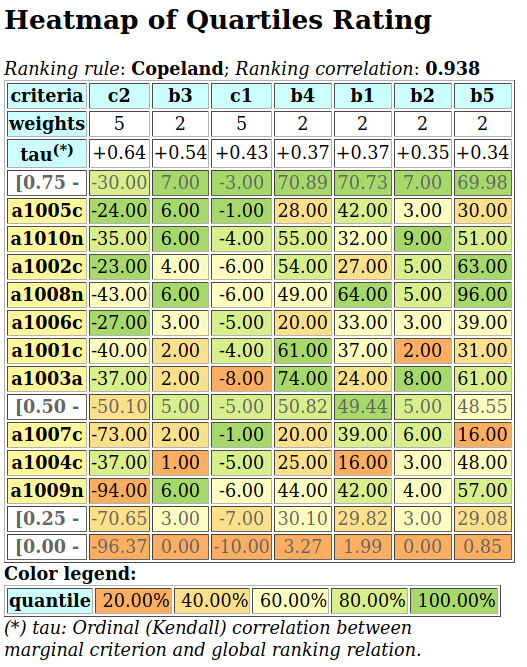
\includegraphics[width=7cm]{Figures/heatMap1.png}
\caption{Heatmap of absolute quartiles ranking. The quartile equivalence classes appear lower-closed. No alternative is rated into the \texttt{Q1} class ($[0.00 - 0.25[$) and no alternative is rated into the Q4 class ($[0.75 - 1.00]$). }
\label{fig:10.2}       % Give a unique label
\end{figure}
	    
Using furthermore a specialised version of the \texttt{exportGraphViz()} method allows drawing the same rating result in a Hasse diagram format (see Fig. \ref{fig:10.3}).
\begin{lstlisting}
>>> lqr.exportRatingGraphViz('normedRatingDigraph')
 *---- exporting a dot file for GraphViz tools ---------*
  Exporting to normedRatingDigraph.dot
  dot -Grankdir=TB -Tpng normedRatingDigraph.dot -o normedRatingDigraph.png
\end{lstlisting}
\begin{figure}[h]
%\sidecaption[t]
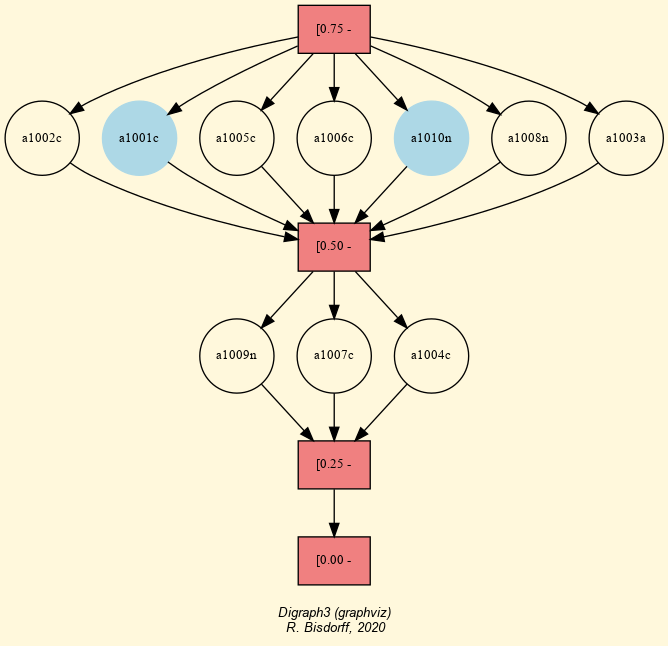
\includegraphics[width=10cm]{Figures/normedRatingDigraph.png}
\caption{Absolute quartiles rating digraph}
\label{fig:10.3}       % Give a unique label
\end{figure}

We may now answer the \emph{absolute rating} problem stated at the beginning. Decision alternatives \texttt{a1001} and \texttt{a1010} (see Table~\ref{tab:10.1}) are both rated into the same third quartile \texttt{Q3} class (see Fig.~\ref{fig:10.3}), even if the \Copeland ranking, obtained from the underlying strict outranking digraph (see Fig.~\ref{fig:10.2}), suggests that alternative \texttt{a1010} is effectively \emph{better performing than} alternative \texttt{a1001}. 

A \emph{preciser} rating result may indeed be achieved when using \emph{deciles} instead of \emph{quartiles} for estimating the historical marginal cumulative distribution functions.
\begin{lstlisting}[caption={Absolute deciles rating result},label=list:10.9]
>>> pq1 = PerformanceQuantiles(pt, numberOfBins = 'deciles',\
...                 LowerClosed=True)
>>> pq1.updateQuantiles(newTab,historySize=None)
>>> lqr1 = LearnedQuantilesRatingDigraph(pq1,newActions,rankingRule='best')
>>> lqr1.showQuantilesRating()
  *-------- Deciles rating result ---------
   [0.60 - 0.70[ ['a1005', 'a1010', 'a1008', 'a1002']
   [0.50 - 0.60[ ['a1006', 'a1001', 'a1003']
   [0.40 - 0.50[ ['a1007', 'a1004']
   [0.30 - 0.40[ ['a1009']
\end{lstlisting}
Compared with the quartiles rating result, we notice in Listing~\ref{list:10.9} that the seven alternatives (\texttt{a1001}, \texttt{a1002}, \texttt{a1003}, \texttt{a1005}, \texttt{a1006}, \texttt{a1008} and \texttt{a1010}), rated before into the third quartile class $[0.50-0.75[$, are now divided up: alternatives \texttt{a1002}, \texttt{a1005}, \texttt{a1008} and \texttt{a1010} attain now the 7th decile class $[0.60-0.70[$, whereas alternatives \texttt{a1001}, \texttt{a1003} and \texttt{a1006} attain only the 6th decile class $[0.50-0.60[$. Of the three \texttt{Q2} $[0.25-0.50[$ rated alternatives (\texttt{a1004}, \texttt{a1007} and \texttt{a1009}), alternatives \texttt{a1004} and \texttt{a1007} are now rated into the 5th decile class $[0.40-0.50[$ and \texttt{a1009} is lowest rated into the 4th decile class $[0.30-0.40[$.

A browser heatmap view may more conveniently illustrate this refined rating result (see Fig.~\ref{fig:10.4}).
\begin{lstlisting}
>>> lqr1.showHTMLRatingHeatmap(\
...       pageTitle='Heatmap of the deciles rating',\
...       colorLevels=5, Correlations=True)
\end{lstlisting}
\begin{figure}[h]
\sidecaption[t]
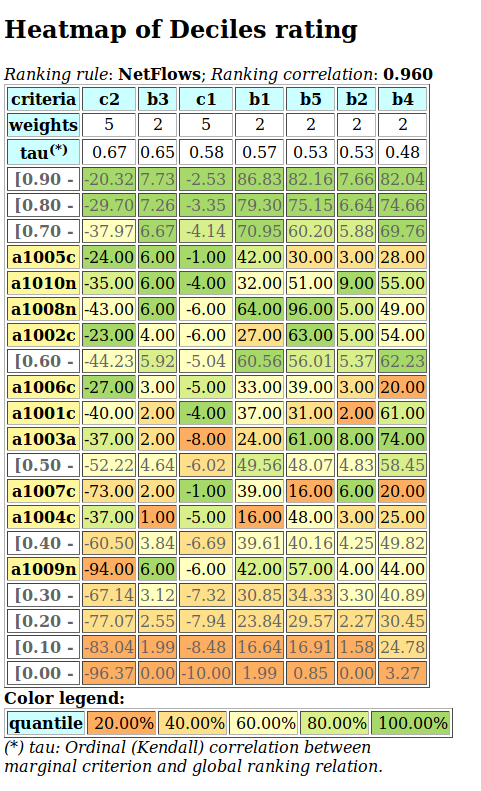
\includegraphics[width=7cm]{Figures/heatMap2.png}
\caption{Heatmap of absolute deciles rating. Decision alternatives \texttt{a1001} and \texttt{a1010} are now, as expected, rated in the $6^{th}$ decile (\texttt{D6}), respectively in the $7^{th}$ decile (\texttt{D7}).}
\label{fig:10.4}       % Give a unique label
\end{figure}

To avoid having to recompute performance deciles from historical data when wishing to refine a rating result, it is useful, depending on the actual size of the historical data, to initially compute performance quantiles with a relatively high number of bins, for instance \emph{dodeciles} or even \emph{centiles}. It is then possible to interpolate on the fly \emph{quartiles} or \emph{deciles} for instance, when constructing the rating digraph. 
\begin{lstlisting}[caption={From deciles interpolated quartiles rating result},label=list:10.10]
>>> lqr2 = LearnedQuantilesRatingDigraph(pq1,newActions,
...                   quantiles='quartiles')
>>> lqr2.showQuantilesRating()
  *-------- Deciles rating result ---------
   [0.50 - 0.75[ ['a1005', 'a1010', 'a1002', 'a1008',
                  'a1006', 'a1001', 'a1003']
   [0.25 - 0.50[ ['a1004', 'a1007', 'a1009']
\end{lstlisting}
With the \texttt{quantiles} parameter (see Listing~\ref{list:10.10} Line 2), we may recover by interpolation the same quartiles rating as obtained directly with historical performance quartiles (see Listing~\ref{list:10.8}). Mind that a correct interpolation of quantiles from a given cumulative distribution function requires more or less uniform distributions of observations in each bin. 

More generally, in the case of industrial production monitoring problems, for instance, where large volumes of historical performance data may be available, it may be of interest to estimate even more precisely the marginal cumulative distribution functions, especially when \emph{tail} rating results, i.e. distinguishing \emph{very best}, or \emph{very weak} multiple criteria performances, become a critical issue. Similarly, the \texttt{historySize} parameter may be used for monitoring on the fly \emph{unstable} random multiple criteria performance data.  	

%%%%%%%
%The chapter bibliography
%\normallatexbib
\clearpage
%\phantomsection
%\addcontentsline{toc}{chapter}{Chapter Bibliography}
\bibliographystyle{spbasic}
%\typeout{}
\bibliography{03-backMatters/reference}
%\chapter{Rating by ranking with learned performance quantile norms}
\label{sec:10}

\abstract*{ We address in Chapter~\ref{sec:10} the problem of rating multiple-criteria performances of a set of potential decision alternatives with respect to performance quantiles learned from historical performance data gathered from similar decision alternatives observed in the past. We show how to learn performance quantiles from historical performance tableaux. New performance records may now be rated with respect to these quantile norms.}

\abstract{ We address in Chapter~\ref{sec:10} the problem of rating multiple-criteria performances of a set of potential decision alternatives with respect to performance quantiles learned from historical performance data gathered from similar decision alternatives observed in the past. We show how to learn performance quantiles from historical performance tableaux. New performance records may now be rated with respect to these quantile norms.}

\section{The absolute rating problem}
\label{sec:10.1}
	  
To illustrate the \emph{absolute rating} problem we face, consider for a moment that, in a given decision making problem we observe, for instance, in Table~\vref{tab:10.1} below, the multi-criteria performance evaluations of two potential decision alternatives, named \texttt{a1001} and \texttt{a1010}, evaluated on 7 \emph{incommensurable} performance criteria: 2 \emph{Costs} criteria \texttt{c1} and \texttt{c2} (to \emph{minimise}) and 5 \emph{Benefits} criteria \texttt{b1} to \texttt{b5} (to \emph{maximise}). 
\begin{table}[ht]
\caption{Multi-criteria performances of two potential decision alternatives}
\label{tab:10.1}       % Give a unique label
\begin{center}
  %\begin{small}
    \begin{tabular}{l|c|c|c|c|c|c|c}
      \svhline\noalign{\smallskip}
      Criterion (weight) & \texttt{b1} (2) & \texttt{b2} (2) & \texttt{b3} (2) & \texttt{b4} (2) & \texttt{b5} (2) & \texttt{c1} (5) & \texttt{c2} (5)\\
      \noalign{\smallskip}\hline\noalign{\smallskip}
    \texttt{a1001} &   37.0  &  2 & 2 & 61.0 & 31.0 & -4 & -40.0\\
    \texttt{a1010} &   32.0 & 9 & 6 & 55.0 & 51.0 & -4 & -35.0 \\
      \noalign{\smallskip}\hline
    \end{tabular}
  %\end{small}
\end{center}
\end{table}

The performance on \emph{Benefits} criteria \texttt{b1}, \texttt{b4} and \texttt{b5} is measured on a cardinal scale from $0.0$ (worst) to $100.0$ (best) whereas, the performance on the \emph{Benefits} criteria \texttt{b2} and \texttt{b3}  and on the \emph{Costs} criterion \texttt{c1} is measured on an ordinal scale from $0$ (worst) to $10$ (best), respectively $-10$ (worst) to $0$ (best). The performance on the \emph{Costs} criterion \texttt{c2} is eventually measured on a cardinal \emph{negative} scale from $-100.00$ (worst) to $0.0$ (best). The two \emph{Costs} criteria are equi-significant (weight 5). Similarly, the five Benefits criteria are also equi-significant (weight 2). The \emph{importance} (sum of significance weights: $2 \times 5 = 10$) of the \emph{Costs} criteria is hence \emph{equivalent} to the \emph{importance} (sum of significance weights: $5 \times 2 = 10$) of the \emph{Benefits} criteria.
   
The non trivial decision problem we now face, is to decide, how the previous two multiple-criteria performance records of alternatives \texttt{a1001}, respectively \texttt{a1010},  may be rated: \emph{excellent}~? \emph{good}~?, or \emph{fair}~?; perhaps even, \emph{weak}~? or \emph{very weak}~? when compared with similar multi-criteria performance records one has already rated into quantiles in the past. 

To solve this \emph{absolute} rating problem, first, we need to estimate multi-criteria \emph{performance quantiles} from historical records \citep{CPSTAT-L5}.  

\section{Incremental learning of historical performance quantiles}
\label{sec:10.2}

Suppose that we see flying in random multiple-criteria performances from a given model of random performance tableau (see Chap.~\ref{sec:5}). The question we address here is to estimate empirical performance quantiles on the basis of so far observed performance vectors. For this task, we are inspired by \citet*{CHAM-2006}, who present an efficient algorithm for incrementally updating a quantile-binned cumulative distribution function (CDF) with newly observed CDFs\footnote{We have adapted in Python a C++ implementation published by \citep*[Chapter 5]{NR3-2007}.}. 

The \texttt{PerformanceQuantiles}\index{PerformanceQuantiles@\texttt{PerformanceQuantiles} class} class, using the \texttt{IncrementalQuan\-tiles\-Estimator} class\index{IncrementalQuantilesEstimator@\texttt{IncrementalQuantilesEstimator} class} from the \texttt{randomNumbers} module \index{randomNumbers@\texttt{randomNumbers} module}, implements such a performance quantiles estimation based on a given performance tableau \citep{BIS-2021b}.

Its main attributes are:
\begin{itemize}[rightmargin=0.5cm,leftmargin=0.5cm,topsep=1pt]
\item Ordered \texttt{objectives} and a \texttt{criteria} dictionaries from a valid performance tableau instance;
\item A list \texttt{quantileFrequencies} of quantile frequencies like:
  \begin{itemize}[nosep]
  \item \emph{quartiles} $[0.0, 0.25, 05, 0.75,1.0]$,
  \item  \emph{quintiles} $[0.0, 0.2, 0.4, 0.6, 0.8, 1.0]$ or
  \item  \emph{deciles} $[0.0, 0.1, 0.2, ... 1.0]$ for instance;
  \end{itemize}
\item An ordered  dictionary \texttt{limitingQuantiles} of so far estimated \emph{lower} (default) or \emph{upper} quantile class limits for each frequency per criterion;
\item An ordered dictionary \texttt{historySizes} for keeping track of the number of evaluations seen so far per criterion. Missing data, the case given, make these sizes vary from criterion to criterion.
\end{itemize}

Below, we show an example Python session concerning 900 decision alternatives randomly generated with a \emph{Cost-Benefit} performance tableau model (see Sec.~\ref{sec:5.3}) from which are also drawn the performances of alternatives \texttt{a1001} and \texttt{a1010} shown in Table~\vref{tab:10.1} above.
\begin{lstlisting}[caption={Computing performance quantiles from a given performance tableau},label=list:10.1]
>>> from performanceQuantiles import PerformanceQuantiles
>>> from randomPerfTabs import RandomCBPerformanceTableau
>>> nbrActions=900
>>> nbrCrit = 7
>>> seed = 100
>>> pt = RandomCBPerformanceTableau(numberOfActions=nbrActions,\
...                  numberOfCriteria=nbrCrit,seed=seed)
>>> pq = PerformanceQuantiles(pt,\
...                   numberOfBins = 'quartiles',\
...                   LowerClosed=True)
>>> pq
  *------- PerformanceQuantiles instance description ------*
   Instance class   : PerformanceQuantiles
   Instance name    : 4-tiled_performances
   Objectives       : 2
   Criteria         : 7
   Quantiles        : 4
   History sizes    : {'c1': 887,'b1': 888,'b2': 891,'b3': 895,
                        'b4': 892,'c2': 893,'b5': 887}
   Attributes       : ['perfTabType','valueDigits',
                       'actionsTypeStatistics',
                       'objectives', 'BigData',
                       'missingDataProbability',
		       'criteria', 'LowerClosed', 'name',
		       'quantilesFrequencies', 'historySizes',
		       'limitingQuantiles', 'cdf']
\end{lstlisting}
The \texttt{PerformanceQuantiles} class parameter \texttt{numberOfBins} (see List.~\vref{list:10.1} Line 9 above), choosing the wished number of quantile frequencies, may be either \emph{quartiles} (4 bins), \emph{quintiles} (5 bins), \emph{deciles} (10 bins), \emph{dodeciles} (20 bins) or any other integer number of quantile bins. The quantile bins may be either \emph{lower closed} (default) or \emph{upper-closed}.

Inspecting the estimated quartile limits may be operated with the\\ \texttt{showLimitingQuantiles()} method.\index{showLimitingQuantiles@\texttt{showLimitingQuantiles()}}
\begin{lstlisting}[caption={Printing out the estimated quartile limits},label=list:10.2]
>>> pq.showLimitingQuantiles(ByObjectives=True)
    ----  Historical performance quantiles -----*
    Costs
    criteria | weights |  '0.00' '0.25' '0.50' '0.75' '1.00'   
    ---------|----------------------------------------------------
       'c1'  |    5    |   -10    -7     -5     -3      0  
       'c2'  |    5    | -96.37 -70.65 -50.10 -30.00  -1.43  
    Benefits
    criteria | weights | '0.00'  '0.25' '0.50' '0.75' '1.00'   
    ---------|-----------------------------------------------------
       'b1'  |    2    |  1.99    29.82 49.44  70.73  99.83  
       'b2'  |    2    |    0      3      5      7     10  
       'b3'  |    2    |    0      3      5      7     10  
       'b4'  |    2    |  3.27   30.10  50.82  70.89  98.05  
       'b5'  |    2    |  0.85   29.08  48.55  69.98  97.56  
\end{lstlisting}
Both objectives are \emph{equally important}; the sum of weights (10) of the \emph{Costs} criteria balance the sum of weights (10) of the \emph{Benefits} criteria (see List.~\vref{list:10.2} column 2). The preference direction of the \emph{Costs} criteria \texttt{c1} and \texttt{c2} is \emph{negative}; the lesser the costs, the better it is, whereas all the \emph{Benefits} criteria \texttt{b1} to \texttt{b5} show \emph{positive} preference directions, i.e. the higher the benefits, the better it is. The columns entitled '$0.00$', resp. '$1.00$' show the \emph{quartile} \texttt{Q0}, resp. \texttt{Q4}, i.e. the \emph{worst}, resp. \emph{best} performance observed so far on each criterion. Column '$0.50$' shows the \emph{median} (\texttt{Q2}) performance observed on the criteria.  

New  decision alternatives with random multiple-criteria performance vectors from the same random performance tableau model as \texttt{pt} (see List.~\vref{list:10.1}) may now be generated with a generic \texttt{RandomPerformanceGenerator} class\index{RandomPerformanceGenerator@\texttt{RandomPerformanceGenerator()}} from the \texttt{randomPerfTabs} module \citep{BIS-2021b}.\footnote{The \texttt{RandomPerformanceGenerator} class works for the \emph{standard} performance tableau model (see Sec.~\ref{sec:5.2}), the \emph{Cost-Benefit} model (see Sec.~\ref{sec:5.3}), and the 3-objectives model (see Sec.~\ref{sec:5.4}).}
\begin{lstlisting}[caption={Generating 100 new random decision alternatives of the same model},label=list:10.3]
>>> from randomPerfTabs import RandomPerformanceGenerator
>>> rpg = RandomPerformanceGenerator(tp,seed=seed)
>>> newTab = rpg.randomPerformanceTableau(100)
\end{lstlisting}

The so far estimated historical quantile limits must, first, be updated with this newly arriving 100 data records:
\begin{lstlisting}
>>> # Updating the quartile norms shown above 
>>> pq.updateQuantiles(newTab,historySize=None)
\end{lstlisting}
Parameter \texttt{historySize} of the \texttt{updateQuantiles()} method\index{updateQuantiles@\texttt{updateQuantiles()}} (Line 2 above) allows to \emph{balance} the \emph{new} evaluations against the \emph{historical} ones.

With \texttt{historySize = None} (the default setting), the balance in the example above is $900/1000$ ($90\%$, the weight of historical data) against $100/1000$ ($10\%$, the weight of the new incoming observations). Setting \texttt{historySize = 0}, for instance, will ignore all historical data ($0/100$ against $100/100$) and restart building the quantile estimation with solely the new incoming data. The \texttt{showHTMLLimitingQuantiles()} method\index{showHTMLLimitingQuantiles@\texttt{showHTMLLimitingQuantiles()}} shows the updated quantile limits in a browser view (see Fig.~\vref{fig:10.1}).
\begin{lstlisting}
>>> # showing the updated quantile limits in a browser view
>>> pq.showHTMLLimitingQuantiles(Transposed=True)
\end{lstlisting}
\begin{figure}[ht]
\sidecaption[t]
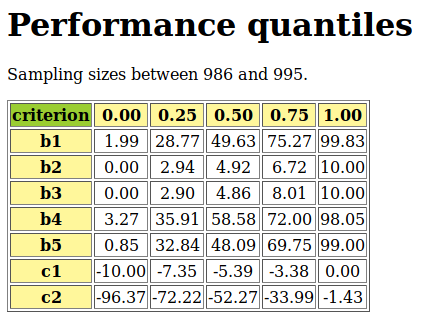
\includegraphics[width=7cm]{Figures/10-1-examplePerfQuantiles.png}
\caption[Showing updated quartiles limits per criterion]{\emph{Showing updated quartiles limits per criterion}. The $0.25$ column shows the first quartile (\texttt{Q1}) limits, the $0.50$ column shows the second quartile (\texttt{Q2}) limits and the $0.75$ column shows the third quartile (\texttt{Q3}) limits. Column $0.00$ (resp. $1.00$) shows the minimum (resp. maximum) performance on each criterion}
\label{fig:10.1}       % Give a unique label
\end{figure}
    
\section{Rating-by-ranking new performances with quantile norms}
\label{sec:10.3}

For \emph{rating} a newly given set of decision alternatives with the help of empirical performance quantiles estimated from historical data, the \texttt{sortingDigraphs} module provides the \texttt{Learned\-QuantilesRatingDigraph} class\index{LearnedQuantilesRatingDigraph@\texttt{LearnedQuantilesRatingDigraph} class}, a specialisation of the \texttt{QuantilesSor\-tingDigraph} class (see Chap.~\ref{sec:9}). The absolute rating result is computed by \emph{ranking} the new performance records together with the learned historical quantile limits.

The class constructor requires a valid \texttt{PerformanceQuantiles} instance and, by default, uses the \Copeland or the \NetFlows ranking rule, whichever fits best in an ordinal correlation sense with the underlying outranking digraph.

It is important to notice that the \texttt{LearnedQuantilesRatingDigraph} class, contrary to the generic \texttt{OutrankingDigraph} class, does not inherit from the generic \texttt{PerformanceTableau} class, but instead from the \texttt{Performance\-Quantiles} class \citep{BIS-2021b}.

The \texttt{actions} attribute in such a \texttt{LearnedQuantilesRatingDigraph} class instance contains not only the newly given decision alternatives, but also the historical quantile limits (attribute \texttt{profiles}) obtained from a given \texttt{Perfor\-manceQuantiles} class instance, i.e. estimated quantile bins' performance limits from historical performance data.

We reconsider now the \texttt{PerformanceQuantiles} object instance \texttt{pq} as computed in the previous section. Let \texttt{newActions} be a list of 10 new decision alternatives generated with the same random performance tableau generator \texttt{rpq} and including, for our didactical purpose, the two decision alternatives \texttt{a1001} and \texttt{a1010} mentioned at the beginning.
\begin{lstlisting}[caption={Computing the absolute rating of 10 new decision alternatives},label=list:10.4]
>>> from sortingDigraphs import LearnedQuantilesRatingDigraph
>>> newActions = rpg.randomActions(10)
>>> lqr = LearnedQuantilesRatingDigraph(pq,newActions,\
...                                     rankingRule='best')
>>> lqr
  *---- Object instance description
   Instance class      : LearnedQuantilesRatingDigraph
   Instance name       : normedRatingDigraph
   Criteria            : 7
   Quantile profiles   : 4
   Lower-closed bins   : True
   New actions         : 10
   Size                : 93
   Determinateness (%) : 76.1
   Ranking rule        : Copeland
   Ordinal correlation : +0.95
   Attributes: ['runTimes','objectives','criteria',
     'LowerClosed','quantilesFrequencies',
     'limitingQuantiles','historySizes','cdf','name',
     'newActions','evaluation','categories',
     'criteriaCategoryLimits','profiles','profileLimits',
     'hasNoVeto','actions','completeRelation','relation',
     'concordanceRelation','valuationdomain','order',
     'gamma','notGamma','rankingRule','rankingCorrelation',
     'rankingScores','actionsRanking','ratingCategories',
     'ratingRelation','relationOrig']
  *---- Constructor run times (in sec.)
   Threads           : 1
   Total time       : 0.02218
   Data input       : 0.00134
   Quantile classes : 0.00008
   Compute profiles : 0.00021
   Compute relation : 0.01869
   Compute rating   : 0.00186
   Compute sorting  : 0.00000
\end{lstlisting}

Data input to the \texttt{LearnedQuantilesRatingDigraph} class constructor are a valid \texttt{PerformanceQuantiles} object \texttt{pq} and a \texttt{newActions} list of newly generated decision alternatives with the same random generator \texttt{rpg} (see List.~\vref{list:10.4} Line 2-3).

The \texttt{actionsSubset} parameter of the \texttt{showPerformanceTableau()} method\index{showPerformanceTableau@\texttt{showPerformanceTableau()}} allows a look at the digraph's nodes, here called \texttt{newActions}.
\begin{lstlisting}[caption={Performance tableau of the new incoming decision alternatives},label=list:10.5,basicstyle=\ttfamily\scriptsize]
>>> lqr.showPerformanceTableau(actionsSubset=lqr.newActions)
 *----  performance tableau -----*
 criteria | a1001 a1002 a1003 a1004 a1005 a1006 a1007 a1008 a1009 a1010   
 ---------|-------------------------------------------------------------
    'b1'  |  37.0  27.0  24.0  16.0  42.0  33.0  39.0  64.0  42.0  32.0  
    'b2'  |   2.0   5.0   8.0   3.0   3.0   3.0   6.0   5.0   4.0   9.0  
    'b3'  |   2.0   4.0   2.0   1.0   6.0   3.0   2.0   6.0   6.0   6.0  
    'b4'  |  61.0  54.0  74.0  25.0  28.0  20.0  20.0  49.0  44.0  55.0  
    'b5'  |  31.0  63.0  61.0  48.0  30.0  39.0  16.0  96.0  57.0  51.0  
    'c1'  |  -4.0  -6.0  -8.0  -5.0  -1.0  -5.0  -1.0  -6.0  -6.0  -4.0  
    'c2'  | -40.0 -23.0 -37.0 -37.0 -24.0 -27.0 -73.0 -43.0 -94.0 -35.0  
\end{lstlisting}

Among the 10 new incoming decision alternatives, we recognise alternatives \texttt{a1001} (see column 2) and \texttt{a1010} (see last column) we have shown in Table~\vref{tab:10.1}.

The \texttt{actions} dictionary of a \texttt{LearnedQuantilesRatingDigraph} class instance includes, besides the 10 performance evaluations of the ten new alternatives, also the closed lower limits of the four quartile classes: \texttt{m1} = $[0.0- [$, \texttt{m2} = $[0.25- [$, \texttt{m3} = $[0.5- [$, \texttt{m4} = $[0.75 - [$. We find these limits in the \texttt{profiles} attribute (see List.~\vref{list:10.6} below).
\begin{lstlisting}[caption={Showing the limiting profiles of the rating quantiles},label=list:10.6]
>>> lqr.showPerformanceTableau(actionsSubset=lqr.profiles)
    *----  Quartiles limit profiles -----*
    criteria |  'm1'   'm2'   'm3'   'm4'   
    ---------|----------------------------
       'b1'  |  2.0    28.8   49.6   75.3  
       'b2'  |  0.0     2.9    4.9    6.7  
       'b3'  |  0.0     2.9    4.9    8.0  
       'b4'  |  3.3    35.9   58.6   72.0  
       'b5'  |  0.8    32.8   48.1   69.7  
       'c1'  | -10.0   -7.4   -5.4   -3.4  
       'c2'  | -96.4  -72.2  -52.3  -34.0  
\end{lstlisting}

The main run time is spent by the \texttt{LearnedQuantilesRatingDigraph} class constructor in computing a bipolar-valued outranking relation on the extended actions set including both the new alternatives as well as the quartile class limits (see List.~\vref{list:10.4} Lines 23-29).\footnote{In case of large volumes, i.e. many new decision alternatives and centile classes for instance, a multi-threading version may be used when multiple processing cores are available \citep{BIS-2021b}.}

The actual rating procedure will rely on a complete ranking of the new decision alternatives as well as the quantile class limits obtained from the corresponding bipolar-valued outranking digraph. Two efficient and scalable ranking rules, the \Copeland and its valued version, the \NetFlows rule may be used for this purpose. The \texttt{rankingRule} parameter allows to choose one of both. With \texttt{rankingRule='best'} (see List.~\vref{list:10.4} Line 3 ) the \texttt{LearnedQuantiles\-RatingDigraph} constructor will choose the ranking rule that results in the highest ordinal correlation with the given outranking relation (see Chap.~\ref{sec:22} and \citep{BIS-2012a}).

In this rating example, the \Copeland rule appears to be the more appropriate ranking rule.
\begin{lstlisting}[caption={\Copeland ranking of new alternatives and historical quartile limits},label=list:10.7]
>>> lqr.rankingRule
  'Copeland'
>>> lqr.actionsRanking
  ['m4', 'a1005', 'a1010', 'a1002', 'a1008', 'a1006', 'a1001',
   'a1003', 'm3', 'a1007', 'a1004', 'a1009', 'm2', 'm1'] 
>>> lqr.showCorrelation(lqr.rankingCorrelation)
  Correlation indexes:
    Crisp ordinal correlation  : +0.945
    Epistemic determination    :  0.522
    Bipolar-valued equivalence : +0.493
\end{lstlisting}

We achieve here in Listing.~\vref{list:10.7} a linear ranking without ties (from best to worst) of the digraph's actions set, i.e. including the new decision alternatives as well as the quartile limits $m1$ to $m4$, which is very close in an ordinal sense ($\tau = 0.945$) to the underlying strict outranking relation.

The eventual rating procedure is based in this example on the \emph{lower} quartile limits, such that the quartile classes' contents are filtered out in increasing order of the \emph{quartiles}.
\begin{lstlisting}
>>> lqr.ratingCategories
 OrderedDict([
 ('m2', ['a1007','a1004','a1009']),
 ('m3', ['a1005','a1010','a1002','a1008',
         'a1006','a1001','a1003'])
 ])
\end{lstlisting}    

We notice above that no new decision alternative is actually rated into the lowest $[0.0-0.25[$, respectively highest $[0.75- [$ quartile classes. Indeed, the absolute rating result is shown with the \texttt{showQuantilesRating()} method\index{showQuantilesRating@\texttt{showQuantilesRating()}}:
\begin{lstlisting}[caption={Absolute quartiles rating result},label=list:10.8]
>>> lqr.showQuantilesRating()
  *-------- Quartiles rating result ---------
   [0.50 - 0.75[ ['a1005', 'a1010', 'a1002', 'a1008',
                  'a1006', 'a1001', 'a1003']
   [0.25 - 0.50[ ['a1007', 'a1004', 'a1009']
\end{lstlisting}    

The same result may also be shown in a browser view with the \texttt{showHTMLRa\-tingHeatmap()} method\index{showHTMLRatingHeatmap@\texttt{showHTMLRatingHeatmap()}} using a specialised rating heatmap format (see Fig.~\vref{fig:10.2}): 
\begin{lstlisting}
>>> lqr.showHTMLRatingHeatmap(\
...            pageTitle='Heatmap of Quartiles Rating',\
...            Correlations=True,colorLevels=5)
\end{lstlisting}
\begin{figure}[ht]
\sidecaption[t]
 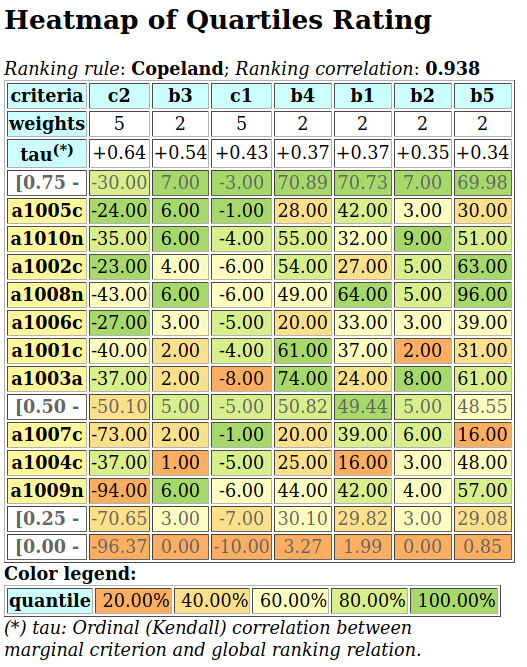
\includegraphics[width=7cm]{Figures/10-2-heatMap1.png}
\caption[Heatmap of absolute quartiles ranking]{\emph{Heatmap of absolute quartiles ranking}. The quartile equivalence classes appear lower-closed. No alternative is rated into the \texttt{Q1} class ($[0.00 - 0.25[$) and no alternative is rated into the Q4 class ($[0.75 - 1.00]$)}
\label{fig:10.2}       % Give a unique label
\end{figure}
	    
Using furthermore a specialised version of the \texttt{exportGraphViz()} method allows drawing in Figure~\vref{fig:10.3} the same rating result in a Hasse diagram format.\footnote{Note that the graphviz dot file was post-edited in order to mark in blue alternatives \texttt{a1001} and \texttt{a1010}.}
\begin{lstlisting}
>>> lqr.exportRatingGraphViz('quartileRatingDigraph')
 *---- exporting a dot file for GraphViz tools ---------*
  Exporting to quartileRatingDigraph.dot
  dot -Grankdir=TB -Tpng quartileRatingDigraph.dot -o quartileRatingDigraph.png
\end{lstlisting}
\begin{figure}[ht]
%\sidecaption[t]
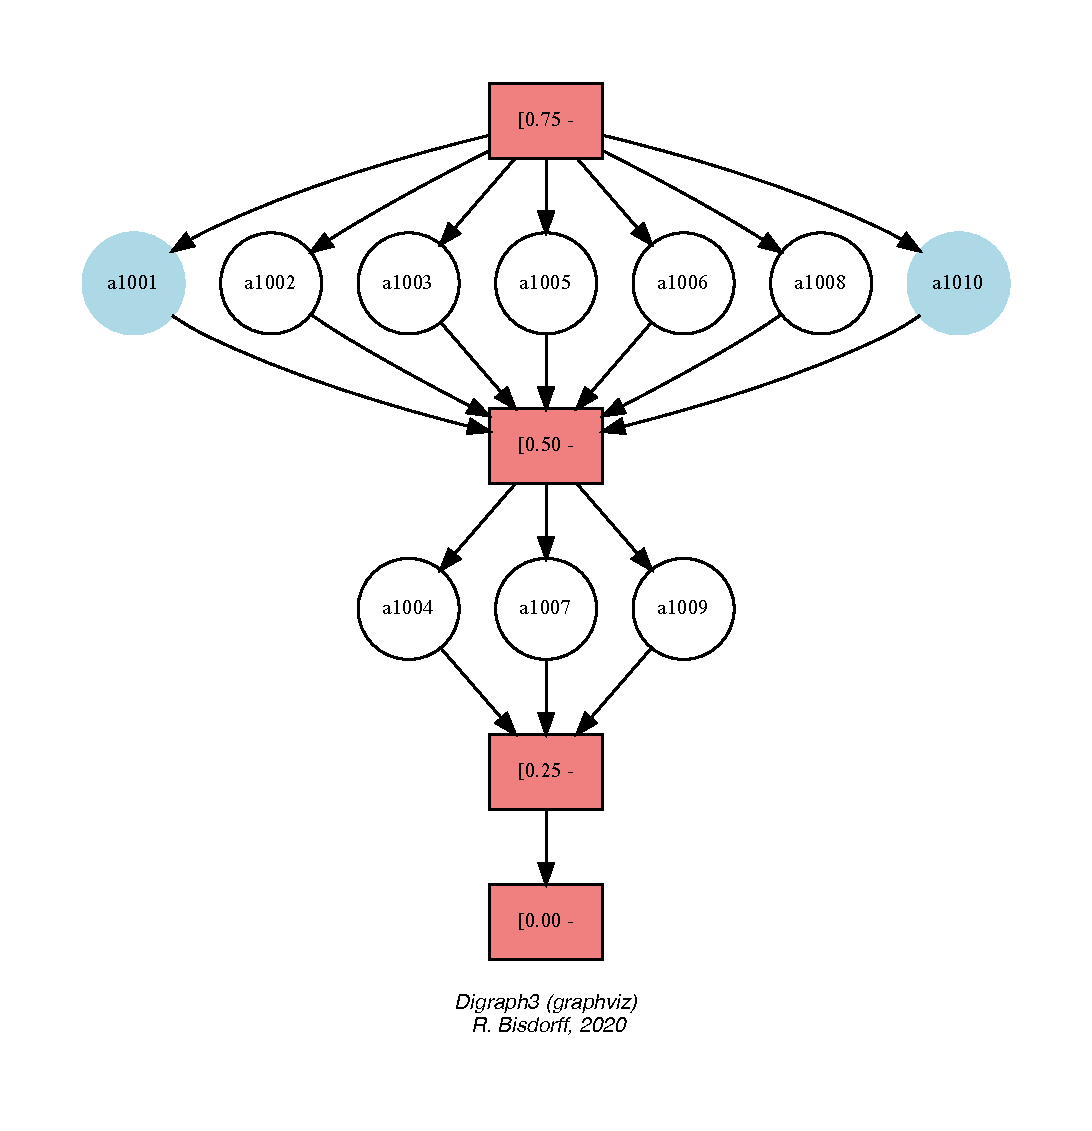
\includegraphics[width=\hsize]{Figures/10-3-normedRatingDigraph.pdf}
\caption{Absolute quartiles rating digraph}
\label{fig:10.3}       % Give a unique label
\end{figure}

We have actually solved now the \emph{absolute rating} problem stated at the beginning. Decision alternatives \texttt{a1001} and \texttt{a1010} (see Tab.~\vref{tab:10.1}) are both rated into the same third quartile \texttt{Q3} class (see Fig.~\vref{fig:10.3}), even if the \Copeland ranking, obtained from the underlying strict outranking digraph (see Fig.~\vref{fig:10.2}), suggests that alternative \texttt{a1010} is effectively \emph{better performing than} alternative \texttt{a1001}. 

A \emph{preciser} rating result may indeed be achieved when using \emph{deciles} instead of \emph{quartiles} for estimating the historical marginal cumulative distribution functions.
\begin{lstlisting}[caption={Absolute deciles rating result},label=list:10.9]
>>> pq1 = PerformanceQuantiles(pt, numberOfBins = 'deciles',\
...                 LowerClosed=True)
>>> pq1.updateQuantiles(newTab,historySize=None)
>>> lqr1 = LearnedQuantilesRatingDigraph(pq1,newActions,rankingRule='best')
>>> lqr1.showQuantilesRating()
  *-------- Deciles rating result ---------
   [0.60 - 0.70[ ['a1005', 'a1010', 'a1008', 'a1002']
   [0.50 - 0.60[ ['a1006', 'a1001', 'a1003']
   [0.40 - 0.50[ ['a1007', 'a1004']
   [0.30 - 0.40[ ['a1009']
\end{lstlisting}

Compared with the quartiles rating result, we notice in Listing~\vref{list:10.9} that the seven alternatives (\texttt{a1001}, \texttt{a1002}, \texttt{a1003}, \texttt{a1005}, \texttt{a1006}, \texttt{a1008} and \texttt{a1010}), rated before into the third quartile class $[0.50-0.75[$, are now divided up: alternatives \texttt{a1002}, \texttt{a1005}, \texttt{a1008} and \texttt{a1010} attain now the 7th decile class $[0.60-0.70[$, whereas alternatives \texttt{a1001}, \texttt{a1003} and \texttt{a1006} attain only the 6th decile class $[0.50-0.60[$. Of the three \texttt{Q2} $[0.25-0.50[$ rated alternatives (\texttt{a1004}, \texttt{a1007} and \texttt{a1009}), alternatives \texttt{a1004} and \texttt{a1007} are now rated into the 5th decile class $[0.40-0.50[$ and \texttt{a1009} is lowest rated into the 4th decile class $[0.30-0.40[$.

A browser heatmap view in Figure~\vref{fig:10.4} more conveniently illustrates this refined rating result.
\begin{lstlisting}
>>> lqr1.showHTMLRatingHeatmap(\
...       pageTitle='Heatmap of the deciles rating',\
...       colorLevels=5, Correlations=True)
\end{lstlisting}
\begin{figure}[ht]
\sidecaption[t]
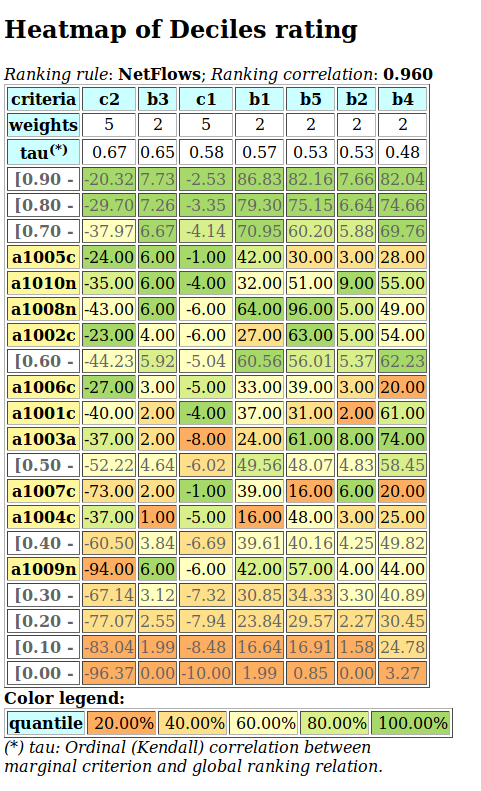
\includegraphics[width=7cm]{Figures/10-4-heatMap2.png}
\caption[Heatmap of absolute deciles rating]{\emph{Heatmap of absolute deciles rating}. Decision alternatives \texttt{a1001} and \texttt{a1010} are now, as expected, rated in the $6^{th}$ decile (\texttt{D6}), respectively in the $7^{th}$ decile (\texttt{D7})}
\label{fig:10.4}       % Give a unique label
\end{figure}

To avoid having to recompute performance deciles from historical data when wishing to refine a rating result, it is useful, depending on the actual size of the historical data, to initially compute performance quantiles with a relatively high number of bins, for instance \emph{dodeciles} or even \emph{centiles}. It is then possible to interpolate on the fly \emph{quartiles} or \emph{deciles} for instance, when constructing the rating digraph. 
\begin{lstlisting}[caption={From deciles interpolated quartiles rating result},label=list:10.10]
>>> lqr2 = LearnedQuantilesRatingDigraph(pq1,newActions,
...                   quantiles='quartiles')
>>> lqr2.showQuantilesRating()
  *-------- Deciles rating result ---------
   [0.50 - 0.75[ ['a1005', 'a1010', 'a1002', 'a1008',
                  'a1006', 'a1001', 'a1003']
   [0.25 - 0.50[ ['a1004', 'a1007', 'a1009']
\end{lstlisting}

With the \texttt{quantiles} parameter (see List.~\vref{list:10.10} Line 2), we recover by interpolation the same quartiles rating as obtained directly with historical performance quartiles (see List.~\vref{list:10.8}). Mind that a correct interpolation of quantiles from a given cumulative distribution function requires more or less uniform distributions of observations in each bin. 
More generally, in the case of industrial production monitoring problems, for instance, where large volumes of historical performance data may be available, it can be of interest to estimate even more precisely the marginal cumulative distribution functions, especially when \emph{tail} rating results, i.e. distinguishing \emph{very best}, or \emph{very weak} multiple-criteria performances, become a critical issue. Similarly, the \texttt{historySize} parameter may be used for monitoring on the fly \emph{unstable} random multiple-criteria performance data \citep{CHAM-2006}.  	

%%%%%%%
%The chapter bibliography
%\normallatexbib
%\clearpage
%\phantomsection
%\addcontentsline{toc}{section}{References}
%\chapter{Rating by ranking with learned performance quantile norms}
\label{sec:10}

\abstract*{ We address in Chapter~\ref{sec:10} the problem of rating multiple-criteria performances of a set of potential decision alternatives with respect to performance quantiles learned from historical performance data gathered from similar decision alternatives observed in the past. We show how to learn performance quantiles from historical performance tableaux. New performance records may now be rated with respect to these quantile norms.}

\abstract{ We address in Chapter~\ref{sec:10} the problem of rating multiple-criteria performances of a set of potential decision alternatives with respect to performance quantiles learned from historical performance data gathered from similar decision alternatives observed in the past. We show how to learn performance quantiles from historical performance tableaux. New performance records may now be rated with respect to these quantile norms.}

\section{The absolute rating problem}
\label{sec:10.1}
	  
To illustrate the \emph{absolute rating} problem we face, consider for a moment that, in a given decision making problem we observe, for instance, in Table~\vref{tab:10.1} below, the multi-criteria performance evaluations of two potential decision alternatives, named \texttt{a1001} and \texttt{a1010}, evaluated on 7 \emph{incommensurable} performance criteria: 2 \emph{Costs} criteria \texttt{c1} and \texttt{c2} (to \emph{minimise}) and 5 \emph{Benefits} criteria \texttt{b1} to \texttt{b5} (to \emph{maximise}). 
\begin{table}[ht]
\caption{Multi-criteria performances of two potential decision alternatives}
\label{tab:10.1}       % Give a unique label
\begin{center}
  %\begin{small}
    \begin{tabular}{l|c|c|c|c|c|c|c}
      \svhline\noalign{\smallskip}
      Criterion (weight) & \texttt{b1} (2) & \texttt{b2} (2) & \texttt{b3} (2) & \texttt{b4} (2) & \texttt{b5} (2) & \texttt{c1} (5) & \texttt{c2} (5)\\
      \noalign{\smallskip}\hline\noalign{\smallskip}
    \texttt{a1001} &   37.0  &  2 & 2 & 61.0 & 31.0 & -4 & -40.0\\
    \texttt{a1010} &   32.0 & 9 & 6 & 55.0 & 51.0 & -4 & -35.0 \\
      \noalign{\smallskip}\hline
    \end{tabular}
  %\end{small}
\end{center}
\end{table}

The performance on \emph{Benefits} criteria \texttt{b1}, \texttt{b4} and \texttt{b5} is measured on a cardinal scale from $0.0$ (worst) to $100.0$ (best) whereas, the performance on the \emph{Benefits} criteria \texttt{b2} and \texttt{b3}  and on the \emph{Costs} criterion \texttt{c1} is measured on an ordinal scale from $0$ (worst) to $10$ (best), respectively $-10$ (worst) to $0$ (best). The performance on the \emph{Costs} criterion \texttt{c2} is eventually measured on a cardinal \emph{negative} scale from $-100.00$ (worst) to $0.0$ (best). The two \emph{Costs} criteria are equi-significant (weight 5). Similarly, the five Benefits criteria are also equi-significant (weight 2). The \emph{importance} (sum of significance weights: $2 \times 5 = 10$) of the \emph{Costs} criteria is hence \emph{equivalent} to the \emph{importance} (sum of significance weights: $5 \times 2 = 10$) of the \emph{Benefits} criteria.
   
The non trivial decision problem we now face, is to decide, how the previous two multiple-criteria performance records of alternatives \texttt{a1001}, respectively \texttt{a1010},  may be rated: \emph{excellent}~? \emph{good}~?, or \emph{fair}~?; perhaps even, \emph{weak}~? or \emph{very weak}~? when compared with similar multi-criteria performance records one has already rated into quantiles in the past. 

To solve this \emph{absolute} rating problem, first, we need to estimate multi-criteria \emph{performance quantiles} from historical records \citep{CPSTAT-L5}.  

\section{Incremental learning of historical performance quantiles}
\label{sec:10.2}

Suppose that we see flying in random multiple-criteria performances from a given model of random performance tableau (see Chap.~\ref{sec:5}). The question we address here is to estimate empirical performance quantiles on the basis of so far observed performance vectors. For this task, we are inspired by \citet*{CHAM-2006}, who present an efficient algorithm for incrementally updating a quantile-binned cumulative distribution function (CDF) with newly observed CDFs\footnote{We have adapted in Python a C++ implementation published by \citep*[Chapter 5]{NR3-2007}.}. 

The \texttt{PerformanceQuantiles}\index{PerformanceQuantiles@\texttt{PerformanceQuantiles} class} class, using the \texttt{IncrementalQuan\-tiles\-Estimator} class\index{IncrementalQuantilesEstimator@\texttt{IncrementalQuantilesEstimator} class} from the \texttt{randomNumbers} module \index{randomNumbers@\texttt{randomNumbers} module}, implements such a performance quantiles estimation based on a given performance tableau \citep{BIS-2021b}.

Its main attributes are:
\begin{itemize}[rightmargin=0.5cm,leftmargin=0.5cm,topsep=1pt]
\item Ordered \texttt{objectives} and a \texttt{criteria} dictionaries from a valid performance tableau instance;
\item A list \texttt{quantileFrequencies} of quantile frequencies like:
  \begin{itemize}[nosep]
  \item \emph{quartiles} $[0.0, 0.25, 05, 0.75,1.0]$,
  \item  \emph{quintiles} $[0.0, 0.2, 0.4, 0.6, 0.8, 1.0]$ or
  \item  \emph{deciles} $[0.0, 0.1, 0.2, ... 1.0]$ for instance;
  \end{itemize}
\item An ordered  dictionary \texttt{limitingQuantiles} of so far estimated \emph{lower} (default) or \emph{upper} quantile class limits for each frequency per criterion;
\item An ordered dictionary \texttt{historySizes} for keeping track of the number of evaluations seen so far per criterion. Missing data, the case given, make these sizes vary from criterion to criterion.
\end{itemize}

Below, we show an example Python session concerning 900 decision alternatives randomly generated with a \emph{Cost-Benefit} performance tableau model (see Sec.~\ref{sec:5.3}) from which are also drawn the performances of alternatives \texttt{a1001} and \texttt{a1010} shown in Table~\vref{tab:10.1} above.
\begin{lstlisting}[caption={Computing performance quantiles from a given performance tableau},label=list:10.1]
>>> from performanceQuantiles import PerformanceQuantiles
>>> from randomPerfTabs import RandomCBPerformanceTableau
>>> nbrActions=900
>>> nbrCrit = 7
>>> seed = 100
>>> pt = RandomCBPerformanceTableau(numberOfActions=nbrActions,\
...                  numberOfCriteria=nbrCrit,seed=seed)
>>> pq = PerformanceQuantiles(pt,\
...                   numberOfBins = 'quartiles',\
...                   LowerClosed=True)
>>> pq
  *------- PerformanceQuantiles instance description ------*
   Instance class   : PerformanceQuantiles
   Instance name    : 4-tiled_performances
   Objectives       : 2
   Criteria         : 7
   Quantiles        : 4
   History sizes    : {'c1': 887,'b1': 888,'b2': 891,'b3': 895,
                        'b4': 892,'c2': 893,'b5': 887}
   Attributes       : ['perfTabType','valueDigits',
                       'actionsTypeStatistics',
                       'objectives', 'BigData',
                       'missingDataProbability',
		       'criteria', 'LowerClosed', 'name',
		       'quantilesFrequencies', 'historySizes',
		       'limitingQuantiles', 'cdf']
\end{lstlisting}
The \texttt{PerformanceQuantiles} class parameter \texttt{numberOfBins} (see List.~\vref{list:10.1} Line 9 above), choosing the wished number of quantile frequencies, may be either \emph{quartiles} (4 bins), \emph{quintiles} (5 bins), \emph{deciles} (10 bins), \emph{dodeciles} (20 bins) or any other integer number of quantile bins. The quantile bins may be either \emph{lower closed} (default) or \emph{upper-closed}.

Inspecting the estimated quartile limits may be operated with the\\ \texttt{showLimitingQuantiles()} method.\index{showLimitingQuantiles@\texttt{showLimitingQuantiles()}}
\begin{lstlisting}[caption={Printing out the estimated quartile limits},label=list:10.2]
>>> pq.showLimitingQuantiles(ByObjectives=True)
    ----  Historical performance quantiles -----*
    Costs
    criteria | weights |  '0.00' '0.25' '0.50' '0.75' '1.00'   
    ---------|----------------------------------------------------
       'c1'  |    5    |   -10    -7     -5     -3      0  
       'c2'  |    5    | -96.37 -70.65 -50.10 -30.00  -1.43  
    Benefits
    criteria | weights | '0.00'  '0.25' '0.50' '0.75' '1.00'   
    ---------|-----------------------------------------------------
       'b1'  |    2    |  1.99    29.82 49.44  70.73  99.83  
       'b2'  |    2    |    0      3      5      7     10  
       'b3'  |    2    |    0      3      5      7     10  
       'b4'  |    2    |  3.27   30.10  50.82  70.89  98.05  
       'b5'  |    2    |  0.85   29.08  48.55  69.98  97.56  
\end{lstlisting}
Both objectives are \emph{equally important}; the sum of weights (10) of the \emph{Costs} criteria balance the sum of weights (10) of the \emph{Benefits} criteria (see List.~\vref{list:10.2} column 2). The preference direction of the \emph{Costs} criteria \texttt{c1} and \texttt{c2} is \emph{negative}; the lesser the costs, the better it is, whereas all the \emph{Benefits} criteria \texttt{b1} to \texttt{b5} show \emph{positive} preference directions, i.e. the higher the benefits, the better it is. The columns entitled '$0.00$', resp. '$1.00$' show the \emph{quartile} \texttt{Q0}, resp. \texttt{Q4}, i.e. the \emph{worst}, resp. \emph{best} performance observed so far on each criterion. Column '$0.50$' shows the \emph{median} (\texttt{Q2}) performance observed on the criteria.  

New  decision alternatives with random multiple-criteria performance vectors from the same random performance tableau model as \texttt{pt} (see List.~\vref{list:10.1}) may now be generated with a generic \texttt{RandomPerformanceGenerator} class\index{RandomPerformanceGenerator@\texttt{RandomPerformanceGenerator()}} from the \texttt{randomPerfTabs} module \citep{BIS-2021b}.\footnote{The \texttt{RandomPerformanceGenerator} class works for the \emph{standard} performance tableau model (see Sec.~\ref{sec:5.2}), the \emph{Cost-Benefit} model (see Sec.~\ref{sec:5.3}), and the 3-objectives model (see Sec.~\ref{sec:5.4}).}
\begin{lstlisting}[caption={Generating 100 new random decision alternatives of the same model},label=list:10.3]
>>> from randomPerfTabs import RandomPerformanceGenerator
>>> rpg = RandomPerformanceGenerator(tp,seed=seed)
>>> newTab = rpg.randomPerformanceTableau(100)
\end{lstlisting}

The so far estimated historical quantile limits must, first, be updated with this newly arriving 100 data records:
\begin{lstlisting}
>>> # Updating the quartile norms shown above 
>>> pq.updateQuantiles(newTab,historySize=None)
\end{lstlisting}
Parameter \texttt{historySize} of the \texttt{updateQuantiles()} method\index{updateQuantiles@\texttt{updateQuantiles()}} (Line 2 above) allows to \emph{balance} the \emph{new} evaluations against the \emph{historical} ones.

With \texttt{historySize = None} (the default setting), the balance in the example above is $900/1000$ ($90\%$, the weight of historical data) against $100/1000$ ($10\%$, the weight of the new incoming observations). Setting \texttt{historySize = 0}, for instance, will ignore all historical data ($0/100$ against $100/100$) and restart building the quantile estimation with solely the new incoming data. The \texttt{showHTMLLimitingQuantiles()} method\index{showHTMLLimitingQuantiles@\texttt{showHTMLLimitingQuantiles()}} shows the updated quantile limits in a browser view (see Fig.~\vref{fig:10.1}).
\begin{lstlisting}
>>> # showing the updated quantile limits in a browser view
>>> pq.showHTMLLimitingQuantiles(Transposed=True)
\end{lstlisting}
\begin{figure}[ht]
\sidecaption[t]
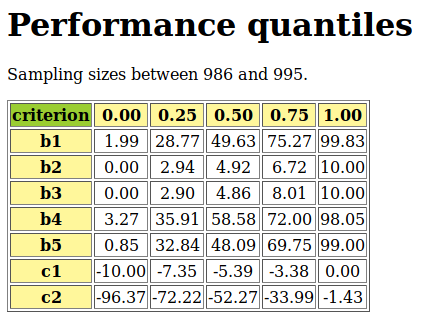
\includegraphics[width=7cm]{Figures/10-1-examplePerfQuantiles.png}
\caption[Showing updated quartiles limits per criterion]{\emph{Showing updated quartiles limits per criterion}. The $0.25$ column shows the first quartile (\texttt{Q1}) limits, the $0.50$ column shows the second quartile (\texttt{Q2}) limits and the $0.75$ column shows the third quartile (\texttt{Q3}) limits. Column $0.00$ (resp. $1.00$) shows the minimum (resp. maximum) performance on each criterion}
\label{fig:10.1}       % Give a unique label
\end{figure}
    
\section{Rating-by-ranking new performances with quantile norms}
\label{sec:10.3}

For \emph{rating} a newly given set of decision alternatives with the help of empirical performance quantiles estimated from historical data, the \texttt{sortingDigraphs} module provides the \texttt{Learned\-QuantilesRatingDigraph} class\index{LearnedQuantilesRatingDigraph@\texttt{LearnedQuantilesRatingDigraph} class}, a specialisation of the \texttt{QuantilesSor\-tingDigraph} class (see Chap.~\ref{sec:9}). The absolute rating result is computed by \emph{ranking} the new performance records together with the learned historical quantile limits.

The class constructor requires a valid \texttt{PerformanceQuantiles} instance and, by default, uses the \Copeland or the \NetFlows ranking rule, whichever fits best in an ordinal correlation sense with the underlying outranking digraph.

It is important to notice that the \texttt{LearnedQuantilesRatingDigraph} class, contrary to the generic \texttt{OutrankingDigraph} class, does not inherit from the generic \texttt{PerformanceTableau} class, but instead from the \texttt{Performance\-Quantiles} class \citep{BIS-2021b}.

The \texttt{actions} attribute in such a \texttt{LearnedQuantilesRatingDigraph} class instance contains not only the newly given decision alternatives, but also the historical quantile limits (attribute \texttt{profiles}) obtained from a given \texttt{Perfor\-manceQuantiles} class instance, i.e. estimated quantile bins' performance limits from historical performance data.

We reconsider now the \texttt{PerformanceQuantiles} object instance \texttt{pq} as computed in the previous section. Let \texttt{newActions} be a list of 10 new decision alternatives generated with the same random performance tableau generator \texttt{rpq} and including, for our didactical purpose, the two decision alternatives \texttt{a1001} and \texttt{a1010} mentioned at the beginning.
\begin{lstlisting}[caption={Computing the absolute rating of 10 new decision alternatives},label=list:10.4]
>>> from sortingDigraphs import LearnedQuantilesRatingDigraph
>>> newActions = rpg.randomActions(10)
>>> lqr = LearnedQuantilesRatingDigraph(pq,newActions,\
...                                     rankingRule='best')
>>> lqr
  *---- Object instance description
   Instance class      : LearnedQuantilesRatingDigraph
   Instance name       : normedRatingDigraph
   Criteria            : 7
   Quantile profiles   : 4
   Lower-closed bins   : True
   New actions         : 10
   Size                : 93
   Determinateness (%) : 76.1
   Ranking rule        : Copeland
   Ordinal correlation : +0.95
   Attributes: ['runTimes','objectives','criteria',
     'LowerClosed','quantilesFrequencies',
     'limitingQuantiles','historySizes','cdf','name',
     'newActions','evaluation','categories',
     'criteriaCategoryLimits','profiles','profileLimits',
     'hasNoVeto','actions','completeRelation','relation',
     'concordanceRelation','valuationdomain','order',
     'gamma','notGamma','rankingRule','rankingCorrelation',
     'rankingScores','actionsRanking','ratingCategories',
     'ratingRelation','relationOrig']
  *---- Constructor run times (in sec.)
   Threads           : 1
   Total time       : 0.02218
   Data input       : 0.00134
   Quantile classes : 0.00008
   Compute profiles : 0.00021
   Compute relation : 0.01869
   Compute rating   : 0.00186
   Compute sorting  : 0.00000
\end{lstlisting}

Data input to the \texttt{LearnedQuantilesRatingDigraph} class constructor are a valid \texttt{PerformanceQuantiles} object \texttt{pq} and a \texttt{newActions} list of newly generated decision alternatives with the same random generator \texttt{rpg} (see List.~\vref{list:10.4} Line 2-3).

The \texttt{actionsSubset} parameter of the \texttt{showPerformanceTableau()} method\index{showPerformanceTableau@\texttt{showPerformanceTableau()}} allows a look at the digraph's nodes, here called \texttt{newActions}.
\begin{lstlisting}[caption={Performance tableau of the new incoming decision alternatives},label=list:10.5,basicstyle=\ttfamily\scriptsize]
>>> lqr.showPerformanceTableau(actionsSubset=lqr.newActions)
 *----  performance tableau -----*
 criteria | a1001 a1002 a1003 a1004 a1005 a1006 a1007 a1008 a1009 a1010   
 ---------|-------------------------------------------------------------
    'b1'  |  37.0  27.0  24.0  16.0  42.0  33.0  39.0  64.0  42.0  32.0  
    'b2'  |   2.0   5.0   8.0   3.0   3.0   3.0   6.0   5.0   4.0   9.0  
    'b3'  |   2.0   4.0   2.0   1.0   6.0   3.0   2.0   6.0   6.0   6.0  
    'b4'  |  61.0  54.0  74.0  25.0  28.0  20.0  20.0  49.0  44.0  55.0  
    'b5'  |  31.0  63.0  61.0  48.0  30.0  39.0  16.0  96.0  57.0  51.0  
    'c1'  |  -4.0  -6.0  -8.0  -5.0  -1.0  -5.0  -1.0  -6.0  -6.0  -4.0  
    'c2'  | -40.0 -23.0 -37.0 -37.0 -24.0 -27.0 -73.0 -43.0 -94.0 -35.0  
\end{lstlisting}

Among the 10 new incoming decision alternatives, we recognise alternatives \texttt{a1001} (see column 2) and \texttt{a1010} (see last column) we have shown in Table~\vref{tab:10.1}.

The \texttt{actions} dictionary of a \texttt{LearnedQuantilesRatingDigraph} class instance includes, besides the 10 performance evaluations of the ten new alternatives, also the closed lower limits of the four quartile classes: \texttt{m1} = $[0.0- [$, \texttt{m2} = $[0.25- [$, \texttt{m3} = $[0.5- [$, \texttt{m4} = $[0.75 - [$. We find these limits in the \texttt{profiles} attribute (see List.~\vref{list:10.6} below).
\begin{lstlisting}[caption={Showing the limiting profiles of the rating quantiles},label=list:10.6]
>>> lqr.showPerformanceTableau(actionsSubset=lqr.profiles)
    *----  Quartiles limit profiles -----*
    criteria |  'm1'   'm2'   'm3'   'm4'   
    ---------|----------------------------
       'b1'  |  2.0    28.8   49.6   75.3  
       'b2'  |  0.0     2.9    4.9    6.7  
       'b3'  |  0.0     2.9    4.9    8.0  
       'b4'  |  3.3    35.9   58.6   72.0  
       'b5'  |  0.8    32.8   48.1   69.7  
       'c1'  | -10.0   -7.4   -5.4   -3.4  
       'c2'  | -96.4  -72.2  -52.3  -34.0  
\end{lstlisting}

The main run time is spent by the \texttt{LearnedQuantilesRatingDigraph} class constructor in computing a bipolar-valued outranking relation on the extended actions set including both the new alternatives as well as the quartile class limits (see List.~\vref{list:10.4} Lines 23-29).\footnote{In case of large volumes, i.e. many new decision alternatives and centile classes for instance, a multi-threading version may be used when multiple processing cores are available \citep{BIS-2021b}.}

The actual rating procedure will rely on a complete ranking of the new decision alternatives as well as the quantile class limits obtained from the corresponding bipolar-valued outranking digraph. Two efficient and scalable ranking rules, the \Copeland and its valued version, the \NetFlows rule may be used for this purpose. The \texttt{rankingRule} parameter allows to choose one of both. With \texttt{rankingRule='best'} (see List.~\vref{list:10.4} Line 3 ) the \texttt{LearnedQuantiles\-RatingDigraph} constructor will choose the ranking rule that results in the highest ordinal correlation with the given outranking relation (see Chap.~\ref{sec:22} and \citep{BIS-2012a}).

In this rating example, the \Copeland rule appears to be the more appropriate ranking rule.
\begin{lstlisting}[caption={\Copeland ranking of new alternatives and historical quartile limits},label=list:10.7]
>>> lqr.rankingRule
  'Copeland'
>>> lqr.actionsRanking
  ['m4', 'a1005', 'a1010', 'a1002', 'a1008', 'a1006', 'a1001',
   'a1003', 'm3', 'a1007', 'a1004', 'a1009', 'm2', 'm1'] 
>>> lqr.showCorrelation(lqr.rankingCorrelation)
  Correlation indexes:
    Crisp ordinal correlation  : +0.945
    Epistemic determination    :  0.522
    Bipolar-valued equivalence : +0.493
\end{lstlisting}

We achieve here in Listing.~\vref{list:10.7} a linear ranking without ties (from best to worst) of the digraph's actions set, i.e. including the new decision alternatives as well as the quartile limits $m1$ to $m4$, which is very close in an ordinal sense ($\tau = 0.945$) to the underlying strict outranking relation.

The eventual rating procedure is based in this example on the \emph{lower} quartile limits, such that the quartile classes' contents are filtered out in increasing order of the \emph{quartiles}.
\begin{lstlisting}
>>> lqr.ratingCategories
 OrderedDict([
 ('m2', ['a1007','a1004','a1009']),
 ('m3', ['a1005','a1010','a1002','a1008',
         'a1006','a1001','a1003'])
 ])
\end{lstlisting}    

We notice above that no new decision alternative is actually rated into the lowest $[0.0-0.25[$, respectively highest $[0.75- [$ quartile classes. Indeed, the absolute rating result is shown with the \texttt{showQuantilesRating()} method\index{showQuantilesRating@\texttt{showQuantilesRating()}}:
\begin{lstlisting}[caption={Absolute quartiles rating result},label=list:10.8]
>>> lqr.showQuantilesRating()
  *-------- Quartiles rating result ---------
   [0.50 - 0.75[ ['a1005', 'a1010', 'a1002', 'a1008',
                  'a1006', 'a1001', 'a1003']
   [0.25 - 0.50[ ['a1007', 'a1004', 'a1009']
\end{lstlisting}    

The same result may also be shown in a browser view with the \texttt{showHTMLRa\-tingHeatmap()} method\index{showHTMLRatingHeatmap@\texttt{showHTMLRatingHeatmap()}} using a specialised rating heatmap format (see Fig.~\vref{fig:10.2}): 
\begin{lstlisting}
>>> lqr.showHTMLRatingHeatmap(\
...            pageTitle='Heatmap of Quartiles Rating',\
...            Correlations=True,colorLevels=5)
\end{lstlisting}
\begin{figure}[ht]
\sidecaption[t]
 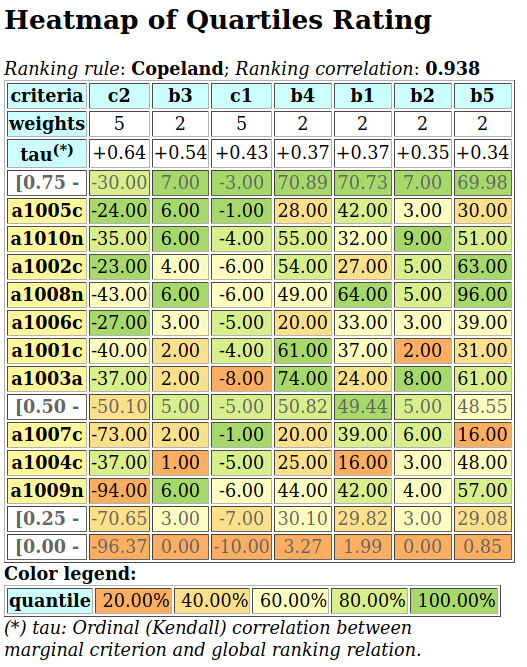
\includegraphics[width=7cm]{Figures/10-2-heatMap1.png}
\caption[Heatmap of absolute quartiles ranking]{\emph{Heatmap of absolute quartiles ranking}. The quartile equivalence classes appear lower-closed. No alternative is rated into the \texttt{Q1} class ($[0.00 - 0.25[$) and no alternative is rated into the Q4 class ($[0.75 - 1.00]$)}
\label{fig:10.2}       % Give a unique label
\end{figure}
	    
Using furthermore a specialised version of the \texttt{exportGraphViz()} method allows drawing in Figure~\vref{fig:10.3} the same rating result in a Hasse diagram format.\footnote{Note that the graphviz dot file was post-edited in order to mark in blue alternatives \texttt{a1001} and \texttt{a1010}.}
\begin{lstlisting}
>>> lqr.exportRatingGraphViz('quartileRatingDigraph')
 *---- exporting a dot file for GraphViz tools ---------*
  Exporting to quartileRatingDigraph.dot
  dot -Grankdir=TB -Tpng quartileRatingDigraph.dot -o quartileRatingDigraph.png
\end{lstlisting}
\begin{figure}[ht]
%\sidecaption[t]
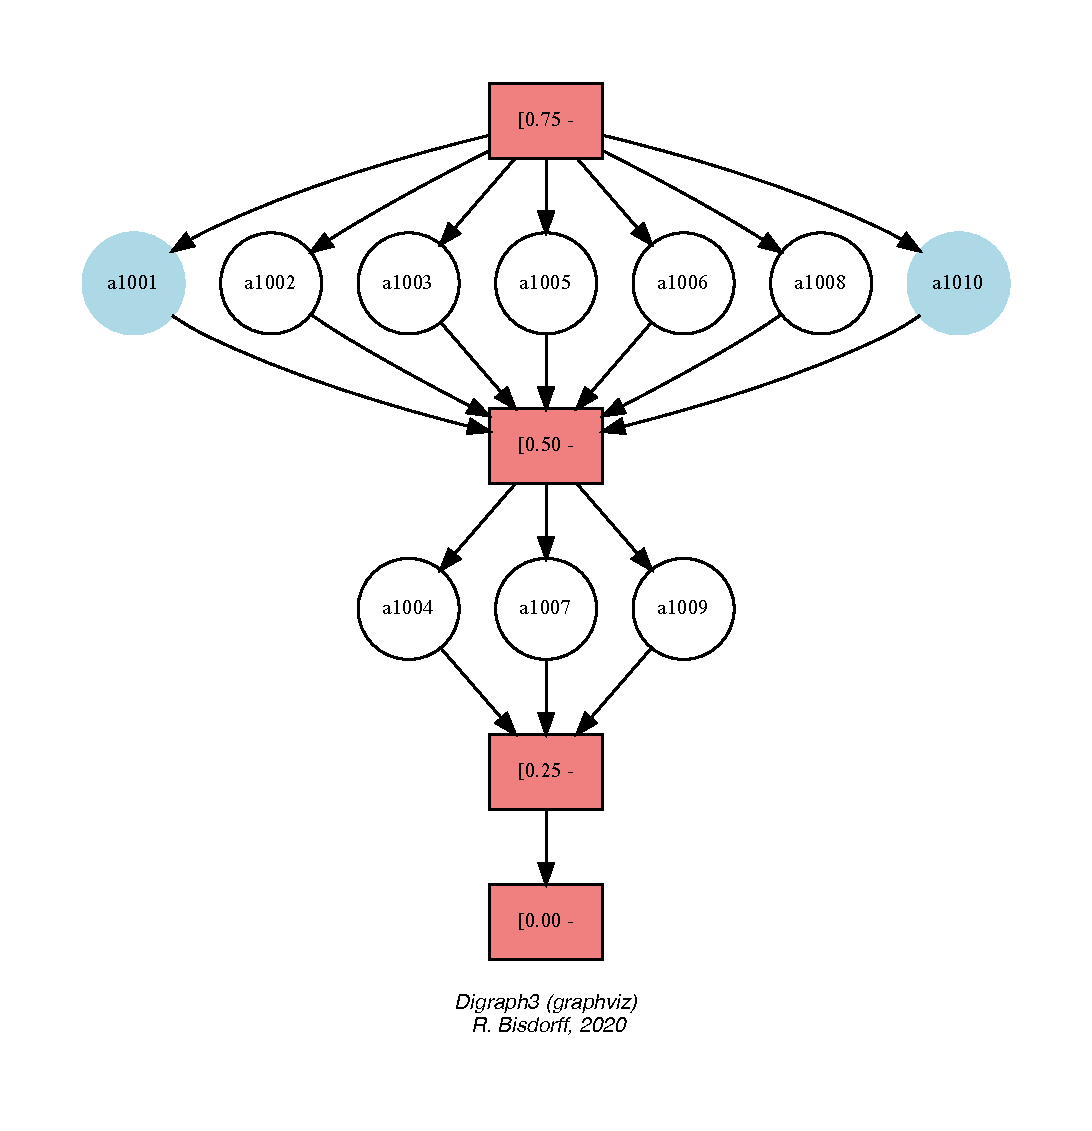
\includegraphics[width=\hsize]{Figures/10-3-normedRatingDigraph.pdf}
\caption{Absolute quartiles rating digraph}
\label{fig:10.3}       % Give a unique label
\end{figure}

We have actually solved now the \emph{absolute rating} problem stated at the beginning. Decision alternatives \texttt{a1001} and \texttt{a1010} (see Tab.~\vref{tab:10.1}) are both rated into the same third quartile \texttt{Q3} class (see Fig.~\vref{fig:10.3}), even if the \Copeland ranking, obtained from the underlying strict outranking digraph (see Fig.~\vref{fig:10.2}), suggests that alternative \texttt{a1010} is effectively \emph{better performing than} alternative \texttt{a1001}. 

A \emph{preciser} rating result may indeed be achieved when using \emph{deciles} instead of \emph{quartiles} for estimating the historical marginal cumulative distribution functions.
\begin{lstlisting}[caption={Absolute deciles rating result},label=list:10.9]
>>> pq1 = PerformanceQuantiles(pt, numberOfBins = 'deciles',\
...                 LowerClosed=True)
>>> pq1.updateQuantiles(newTab,historySize=None)
>>> lqr1 = LearnedQuantilesRatingDigraph(pq1,newActions,rankingRule='best')
>>> lqr1.showQuantilesRating()
  *-------- Deciles rating result ---------
   [0.60 - 0.70[ ['a1005', 'a1010', 'a1008', 'a1002']
   [0.50 - 0.60[ ['a1006', 'a1001', 'a1003']
   [0.40 - 0.50[ ['a1007', 'a1004']
   [0.30 - 0.40[ ['a1009']
\end{lstlisting}

Compared with the quartiles rating result, we notice in Listing~\vref{list:10.9} that the seven alternatives (\texttt{a1001}, \texttt{a1002}, \texttt{a1003}, \texttt{a1005}, \texttt{a1006}, \texttt{a1008} and \texttt{a1010}), rated before into the third quartile class $[0.50-0.75[$, are now divided up: alternatives \texttt{a1002}, \texttt{a1005}, \texttt{a1008} and \texttt{a1010} attain now the 7th decile class $[0.60-0.70[$, whereas alternatives \texttt{a1001}, \texttt{a1003} and \texttt{a1006} attain only the 6th decile class $[0.50-0.60[$. Of the three \texttt{Q2} $[0.25-0.50[$ rated alternatives (\texttt{a1004}, \texttt{a1007} and \texttt{a1009}), alternatives \texttt{a1004} and \texttt{a1007} are now rated into the 5th decile class $[0.40-0.50[$ and \texttt{a1009} is lowest rated into the 4th decile class $[0.30-0.40[$.

A browser heatmap view in Figure~\vref{fig:10.4} more conveniently illustrates this refined rating result.
\begin{lstlisting}
>>> lqr1.showHTMLRatingHeatmap(\
...       pageTitle='Heatmap of the deciles rating',\
...       colorLevels=5, Correlations=True)
\end{lstlisting}
\begin{figure}[ht]
\sidecaption[t]
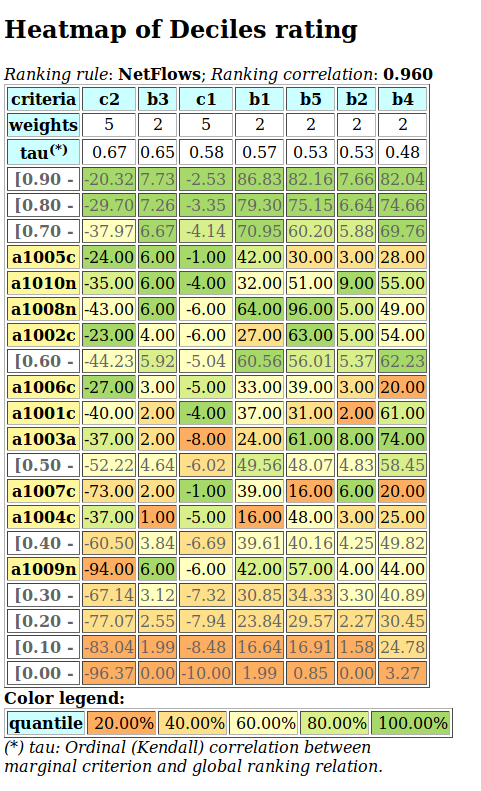
\includegraphics[width=7cm]{Figures/10-4-heatMap2.png}
\caption[Heatmap of absolute deciles rating]{\emph{Heatmap of absolute deciles rating}. Decision alternatives \texttt{a1001} and \texttt{a1010} are now, as expected, rated in the $6^{th}$ decile (\texttt{D6}), respectively in the $7^{th}$ decile (\texttt{D7})}
\label{fig:10.4}       % Give a unique label
\end{figure}

To avoid having to recompute performance deciles from historical data when wishing to refine a rating result, it is useful, depending on the actual size of the historical data, to initially compute performance quantiles with a relatively high number of bins, for instance \emph{dodeciles} or even \emph{centiles}. It is then possible to interpolate on the fly \emph{quartiles} or \emph{deciles} for instance, when constructing the rating digraph. 
\begin{lstlisting}[caption={From deciles interpolated quartiles rating result},label=list:10.10]
>>> lqr2 = LearnedQuantilesRatingDigraph(pq1,newActions,
...                   quantiles='quartiles')
>>> lqr2.showQuantilesRating()
  *-------- Deciles rating result ---------
   [0.50 - 0.75[ ['a1005', 'a1010', 'a1002', 'a1008',
                  'a1006', 'a1001', 'a1003']
   [0.25 - 0.50[ ['a1004', 'a1007', 'a1009']
\end{lstlisting}

With the \texttt{quantiles} parameter (see List.~\vref{list:10.10} Line 2), we recover by interpolation the same quartiles rating as obtained directly with historical performance quartiles (see List.~\vref{list:10.8}). Mind that a correct interpolation of quantiles from a given cumulative distribution function requires more or less uniform distributions of observations in each bin. 
More generally, in the case of industrial production monitoring problems, for instance, where large volumes of historical performance data may be available, it can be of interest to estimate even more precisely the marginal cumulative distribution functions, especially when \emph{tail} rating results, i.e. distinguishing \emph{very best}, or \emph{very weak} multiple-criteria performances, become a critical issue. Similarly, the \texttt{historySize} parameter may be used for monitoring on the fly \emph{unstable} random multiple-criteria performance data \citep{CHAM-2006}.  	

%%%%%%%
%The chapter bibliography
%\normallatexbib
%\clearpage
%\phantomsection
%\addcontentsline{toc}{section}{References}
%\chapter{Rating by ranking with learned performance quantile norms}
\label{sec:10}

\abstract*{ We address in Chapter~\ref{sec:10} the problem of rating multiple-criteria performances of a set of potential decision alternatives with respect to performance quantiles learned from historical performance data gathered from similar decision alternatives observed in the past. We show how to learn performance quantiles from historical performance tableaux. New performance records may now be rated with respect to these quantile norms.}

\abstract{ We address in Chapter~\ref{sec:10} the problem of rating multiple-criteria performances of a set of potential decision alternatives with respect to performance quantiles learned from historical performance data gathered from similar decision alternatives observed in the past. We show how to learn performance quantiles from historical performance tableaux. New performance records may now be rated with respect to these quantile norms.}

\section{The absolute rating problem}
\label{sec:10.1}
	  
To illustrate the \emph{absolute rating} problem we face, consider for a moment that, in a given decision making problem we observe, for instance, in Table~\vref{tab:10.1} below, the multi-criteria performance evaluations of two potential decision alternatives, named \texttt{a1001} and \texttt{a1010}, evaluated on 7 \emph{incommensurable} performance criteria: 2 \emph{Costs} criteria \texttt{c1} and \texttt{c2} (to \emph{minimise}) and 5 \emph{Benefits} criteria \texttt{b1} to \texttt{b5} (to \emph{maximise}). 
\begin{table}[ht]
\caption{Multi-criteria performances of two potential decision alternatives}
\label{tab:10.1}       % Give a unique label
\begin{center}
  %\begin{small}
    \begin{tabular}{l|c|c|c|c|c|c|c}
      \svhline\noalign{\smallskip}
      Criterion (weight) & \texttt{b1} (2) & \texttt{b2} (2) & \texttt{b3} (2) & \texttt{b4} (2) & \texttt{b5} (2) & \texttt{c1} (5) & \texttt{c2} (5)\\
      \noalign{\smallskip}\hline\noalign{\smallskip}
    \texttt{a1001} &   37.0  &  2 & 2 & 61.0 & 31.0 & -4 & -40.0\\
    \texttt{a1010} &   32.0 & 9 & 6 & 55.0 & 51.0 & -4 & -35.0 \\
      \noalign{\smallskip}\hline
    \end{tabular}
  %\end{small}
\end{center}
\end{table}

The performance on \emph{Benefits} criteria \texttt{b1}, \texttt{b4} and \texttt{b5} is measured on a cardinal scale from $0.0$ (worst) to $100.0$ (best) whereas, the performance on the \emph{Benefits} criteria \texttt{b2} and \texttt{b3}  and on the \emph{Costs} criterion \texttt{c1} is measured on an ordinal scale from $0$ (worst) to $10$ (best), respectively $-10$ (worst) to $0$ (best). The performance on the \emph{Costs} criterion \texttt{c2} is eventually measured on a cardinal \emph{negative} scale from $-100.00$ (worst) to $0.0$ (best). The two \emph{Costs} criteria are equi-significant (weight 5). Similarly, the five Benefits criteria are also equi-significant (weight 2). The \emph{importance} (sum of significance weights: $2 \times 5 = 10$) of the \emph{Costs} criteria is hence \emph{equivalent} to the \emph{importance} (sum of significance weights: $5 \times 2 = 10$) of the \emph{Benefits} criteria.
   
The non trivial decision problem we now face, is to decide, how the previous two multiple-criteria performance records of alternatives \texttt{a1001}, respectively \texttt{a1010},  may be rated: \emph{excellent}~? \emph{good}~?, or \emph{fair}~?; perhaps even, \emph{weak}~? or \emph{very weak}~? when compared with similar multi-criteria performance records one has already rated into quantiles in the past. 

To solve this \emph{absolute} rating problem, first, we need to estimate multi-criteria \emph{performance quantiles} from historical records \citep{CPSTAT-L5}.  

\section{Incremental learning of historical performance quantiles}
\label{sec:10.2}

Suppose that we see flying in random multiple-criteria performances from a given model of random performance tableau (see Chap.~\ref{sec:5}). The question we address here is to estimate empirical performance quantiles on the basis of so far observed performance vectors. For this task, we are inspired by \citet*{CHAM-2006}, who present an efficient algorithm for incrementally updating a quantile-binned cumulative distribution function (CDF) with newly observed CDFs\footnote{We have adapted in Python a C++ implementation published by \citep*[Chapter 5]{NR3-2007}.}. 

The \texttt{PerformanceQuantiles}\index{PerformanceQuantiles@\texttt{PerformanceQuantiles} class} class, using the \texttt{IncrementalQuan\-tiles\-Estimator} class\index{IncrementalQuantilesEstimator@\texttt{IncrementalQuantilesEstimator} class} from the \texttt{randomNumbers} module \index{randomNumbers@\texttt{randomNumbers} module}, implements such a performance quantiles estimation based on a given performance tableau \citep{BIS-2021b}.

Its main attributes are:
\begin{itemize}[rightmargin=0.5cm,leftmargin=0.5cm,topsep=1pt]
\item Ordered \texttt{objectives} and a \texttt{criteria} dictionaries from a valid performance tableau instance;
\item A list \texttt{quantileFrequencies} of quantile frequencies like:
  \begin{itemize}[nosep]
  \item \emph{quartiles} $[0.0, 0.25, 05, 0.75,1.0]$,
  \item  \emph{quintiles} $[0.0, 0.2, 0.4, 0.6, 0.8, 1.0]$ or
  \item  \emph{deciles} $[0.0, 0.1, 0.2, ... 1.0]$ for instance;
  \end{itemize}
\item An ordered  dictionary \texttt{limitingQuantiles} of so far estimated \emph{lower} (default) or \emph{upper} quantile class limits for each frequency per criterion;
\item An ordered dictionary \texttt{historySizes} for keeping track of the number of evaluations seen so far per criterion. Missing data, the case given, make these sizes vary from criterion to criterion.
\end{itemize}

Below, we show an example Python session concerning 900 decision alternatives randomly generated with a \emph{Cost-Benefit} performance tableau model (see Sec.~\ref{sec:5.3}) from which are also drawn the performances of alternatives \texttt{a1001} and \texttt{a1010} shown in Table~\vref{tab:10.1} above.
\begin{lstlisting}[caption={Computing performance quantiles from a given performance tableau},label=list:10.1]
>>> from performanceQuantiles import PerformanceQuantiles
>>> from randomPerfTabs import RandomCBPerformanceTableau
>>> nbrActions=900
>>> nbrCrit = 7
>>> seed = 100
>>> pt = RandomCBPerformanceTableau(numberOfActions=nbrActions,\
...                  numberOfCriteria=nbrCrit,seed=seed)
>>> pq = PerformanceQuantiles(pt,\
...                   numberOfBins = 'quartiles',\
...                   LowerClosed=True)
>>> pq
  *------- PerformanceQuantiles instance description ------*
   Instance class   : PerformanceQuantiles
   Instance name    : 4-tiled_performances
   Objectives       : 2
   Criteria         : 7
   Quantiles        : 4
   History sizes    : {'c1': 887,'b1': 888,'b2': 891,'b3': 895,
                        'b4': 892,'c2': 893,'b5': 887}
   Attributes       : ['perfTabType','valueDigits',
                       'actionsTypeStatistics',
                       'objectives', 'BigData',
                       'missingDataProbability',
		       'criteria', 'LowerClosed', 'name',
		       'quantilesFrequencies', 'historySizes',
		       'limitingQuantiles', 'cdf']
\end{lstlisting}
The \texttt{PerformanceQuantiles} class parameter \texttt{numberOfBins} (see List.~\vref{list:10.1} Line 9 above), choosing the wished number of quantile frequencies, may be either \emph{quartiles} (4 bins), \emph{quintiles} (5 bins), \emph{deciles} (10 bins), \emph{dodeciles} (20 bins) or any other integer number of quantile bins. The quantile bins may be either \emph{lower closed} (default) or \emph{upper-closed}.

Inspecting the estimated quartile limits may be operated with the\\ \texttt{showLimitingQuantiles()} method.\index{showLimitingQuantiles@\texttt{showLimitingQuantiles()}}
\begin{lstlisting}[caption={Printing out the estimated quartile limits},label=list:10.2]
>>> pq.showLimitingQuantiles(ByObjectives=True)
    ----  Historical performance quantiles -----*
    Costs
    criteria | weights |  '0.00' '0.25' '0.50' '0.75' '1.00'   
    ---------|----------------------------------------------------
       'c1'  |    5    |   -10    -7     -5     -3      0  
       'c2'  |    5    | -96.37 -70.65 -50.10 -30.00  -1.43  
    Benefits
    criteria | weights | '0.00'  '0.25' '0.50' '0.75' '1.00'   
    ---------|-----------------------------------------------------
       'b1'  |    2    |  1.99    29.82 49.44  70.73  99.83  
       'b2'  |    2    |    0      3      5      7     10  
       'b3'  |    2    |    0      3      5      7     10  
       'b4'  |    2    |  3.27   30.10  50.82  70.89  98.05  
       'b5'  |    2    |  0.85   29.08  48.55  69.98  97.56  
\end{lstlisting}
Both objectives are \emph{equally important}; the sum of weights (10) of the \emph{Costs} criteria balance the sum of weights (10) of the \emph{Benefits} criteria (see List.~\vref{list:10.2} column 2). The preference direction of the \emph{Costs} criteria \texttt{c1} and \texttt{c2} is \emph{negative}; the lesser the costs, the better it is, whereas all the \emph{Benefits} criteria \texttt{b1} to \texttt{b5} show \emph{positive} preference directions, i.e. the higher the benefits, the better it is. The columns entitled '$0.00$', resp. '$1.00$' show the \emph{quartile} \texttt{Q0}, resp. \texttt{Q4}, i.e. the \emph{worst}, resp. \emph{best} performance observed so far on each criterion. Column '$0.50$' shows the \emph{median} (\texttt{Q2}) performance observed on the criteria.  

New  decision alternatives with random multiple-criteria performance vectors from the same random performance tableau model as \texttt{pt} (see List.~\vref{list:10.1}) may now be generated with a generic \texttt{RandomPerformanceGenerator} class\index{RandomPerformanceGenerator@\texttt{RandomPerformanceGenerator()}} from the \texttt{randomPerfTabs} module \citep{BIS-2021b}.\footnote{The \texttt{RandomPerformanceGenerator} class works for the \emph{standard} performance tableau model (see Sec.~\ref{sec:5.2}), the \emph{Cost-Benefit} model (see Sec.~\ref{sec:5.3}), and the 3-objectives model (see Sec.~\ref{sec:5.4}).}
\begin{lstlisting}[caption={Generating 100 new random decision alternatives of the same model},label=list:10.3]
>>> from randomPerfTabs import RandomPerformanceGenerator
>>> rpg = RandomPerformanceGenerator(tp,seed=seed)
>>> newTab = rpg.randomPerformanceTableau(100)
\end{lstlisting}

The so far estimated historical quantile limits must, first, be updated with this newly arriving 100 data records:
\begin{lstlisting}
>>> # Updating the quartile norms shown above 
>>> pq.updateQuantiles(newTab,historySize=None)
\end{lstlisting}
Parameter \texttt{historySize} of the \texttt{updateQuantiles()} method\index{updateQuantiles@\texttt{updateQuantiles()}} (Line 2 above) allows to \emph{balance} the \emph{new} evaluations against the \emph{historical} ones.

With \texttt{historySize = None} (the default setting), the balance in the example above is $900/1000$ ($90\%$, the weight of historical data) against $100/1000$ ($10\%$, the weight of the new incoming observations). Setting \texttt{historySize = 0}, for instance, will ignore all historical data ($0/100$ against $100/100$) and restart building the quantile estimation with solely the new incoming data. The \texttt{showHTMLLimitingQuantiles()} method\index{showHTMLLimitingQuantiles@\texttt{showHTMLLimitingQuantiles()}} shows the updated quantile limits in a browser view (see Fig.~\vref{fig:10.1}).
\begin{lstlisting}
>>> # showing the updated quantile limits in a browser view
>>> pq.showHTMLLimitingQuantiles(Transposed=True)
\end{lstlisting}
\begin{figure}[ht]
\sidecaption[t]
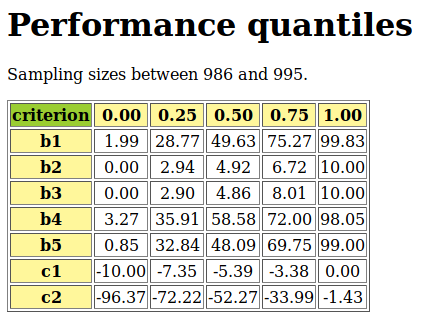
\includegraphics[width=7cm]{Figures/10-1-examplePerfQuantiles.png}
\caption[Showing updated quartiles limits per criterion]{\emph{Showing updated quartiles limits per criterion}. The $0.25$ column shows the first quartile (\texttt{Q1}) limits, the $0.50$ column shows the second quartile (\texttt{Q2}) limits and the $0.75$ column shows the third quartile (\texttt{Q3}) limits. Column $0.00$ (resp. $1.00$) shows the minimum (resp. maximum) performance on each criterion}
\label{fig:10.1}       % Give a unique label
\end{figure}
    
\section{Rating-by-ranking new performances with quantile norms}
\label{sec:10.3}

For \emph{rating} a newly given set of decision alternatives with the help of empirical performance quantiles estimated from historical data, the \texttt{sortingDigraphs} module provides the \texttt{Learned\-QuantilesRatingDigraph} class\index{LearnedQuantilesRatingDigraph@\texttt{LearnedQuantilesRatingDigraph} class}, a specialisation of the \texttt{QuantilesSor\-tingDigraph} class (see Chap.~\ref{sec:9}). The absolute rating result is computed by \emph{ranking} the new performance records together with the learned historical quantile limits.

The class constructor requires a valid \texttt{PerformanceQuantiles} instance and, by default, uses the \Copeland or the \NetFlows ranking rule, whichever fits best in an ordinal correlation sense with the underlying outranking digraph.

It is important to notice that the \texttt{LearnedQuantilesRatingDigraph} class, contrary to the generic \texttt{OutrankingDigraph} class, does not inherit from the generic \texttt{PerformanceTableau} class, but instead from the \texttt{Performance\-Quantiles} class \citep{BIS-2021b}.

The \texttt{actions} attribute in such a \texttt{LearnedQuantilesRatingDigraph} class instance contains not only the newly given decision alternatives, but also the historical quantile limits (attribute \texttt{profiles}) obtained from a given \texttt{Perfor\-manceQuantiles} class instance, i.e. estimated quantile bins' performance limits from historical performance data.

We reconsider now the \texttt{PerformanceQuantiles} object instance \texttt{pq} as computed in the previous section. Let \texttt{newActions} be a list of 10 new decision alternatives generated with the same random performance tableau generator \texttt{rpq} and including, for our didactical purpose, the two decision alternatives \texttt{a1001} and \texttt{a1010} mentioned at the beginning.
\begin{lstlisting}[caption={Computing the absolute rating of 10 new decision alternatives},label=list:10.4]
>>> from sortingDigraphs import LearnedQuantilesRatingDigraph
>>> newActions = rpg.randomActions(10)
>>> lqr = LearnedQuantilesRatingDigraph(pq,newActions,\
...                                     rankingRule='best')
>>> lqr
  *---- Object instance description
   Instance class      : LearnedQuantilesRatingDigraph
   Instance name       : normedRatingDigraph
   Criteria            : 7
   Quantile profiles   : 4
   Lower-closed bins   : True
   New actions         : 10
   Size                : 93
   Determinateness (%) : 76.1
   Ranking rule        : Copeland
   Ordinal correlation : +0.95
   Attributes: ['runTimes','objectives','criteria',
     'LowerClosed','quantilesFrequencies',
     'limitingQuantiles','historySizes','cdf','name',
     'newActions','evaluation','categories',
     'criteriaCategoryLimits','profiles','profileLimits',
     'hasNoVeto','actions','completeRelation','relation',
     'concordanceRelation','valuationdomain','order',
     'gamma','notGamma','rankingRule','rankingCorrelation',
     'rankingScores','actionsRanking','ratingCategories',
     'ratingRelation','relationOrig']
  *---- Constructor run times (in sec.)
   Threads           : 1
   Total time       : 0.02218
   Data input       : 0.00134
   Quantile classes : 0.00008
   Compute profiles : 0.00021
   Compute relation : 0.01869
   Compute rating   : 0.00186
   Compute sorting  : 0.00000
\end{lstlisting}

Data input to the \texttt{LearnedQuantilesRatingDigraph} class constructor are a valid \texttt{PerformanceQuantiles} object \texttt{pq} and a \texttt{newActions} list of newly generated decision alternatives with the same random generator \texttt{rpg} (see List.~\vref{list:10.4} Line 2-3).

The \texttt{actionsSubset} parameter of the \texttt{showPerformanceTableau()} method\index{showPerformanceTableau@\texttt{showPerformanceTableau()}} allows a look at the digraph's nodes, here called \texttt{newActions}.
\begin{lstlisting}[caption={Performance tableau of the new incoming decision alternatives},label=list:10.5,basicstyle=\ttfamily\scriptsize]
>>> lqr.showPerformanceTableau(actionsSubset=lqr.newActions)
 *----  performance tableau -----*
 criteria | a1001 a1002 a1003 a1004 a1005 a1006 a1007 a1008 a1009 a1010   
 ---------|-------------------------------------------------------------
    'b1'  |  37.0  27.0  24.0  16.0  42.0  33.0  39.0  64.0  42.0  32.0  
    'b2'  |   2.0   5.0   8.0   3.0   3.0   3.0   6.0   5.0   4.0   9.0  
    'b3'  |   2.0   4.0   2.0   1.0   6.0   3.0   2.0   6.0   6.0   6.0  
    'b4'  |  61.0  54.0  74.0  25.0  28.0  20.0  20.0  49.0  44.0  55.0  
    'b5'  |  31.0  63.0  61.0  48.0  30.0  39.0  16.0  96.0  57.0  51.0  
    'c1'  |  -4.0  -6.0  -8.0  -5.0  -1.0  -5.0  -1.0  -6.0  -6.0  -4.0  
    'c2'  | -40.0 -23.0 -37.0 -37.0 -24.0 -27.0 -73.0 -43.0 -94.0 -35.0  
\end{lstlisting}

Among the 10 new incoming decision alternatives, we recognise alternatives \texttt{a1001} (see column 2) and \texttt{a1010} (see last column) we have shown in Table~\vref{tab:10.1}.

The \texttt{actions} dictionary of a \texttt{LearnedQuantilesRatingDigraph} class instance includes, besides the 10 performance evaluations of the ten new alternatives, also the closed lower limits of the four quartile classes: \texttt{m1} = $[0.0- [$, \texttt{m2} = $[0.25- [$, \texttt{m3} = $[0.5- [$, \texttt{m4} = $[0.75 - [$. We find these limits in the \texttt{profiles} attribute (see List.~\vref{list:10.6} below).
\begin{lstlisting}[caption={Showing the limiting profiles of the rating quantiles},label=list:10.6]
>>> lqr.showPerformanceTableau(actionsSubset=lqr.profiles)
    *----  Quartiles limit profiles -----*
    criteria |  'm1'   'm2'   'm3'   'm4'   
    ---------|----------------------------
       'b1'  |  2.0    28.8   49.6   75.3  
       'b2'  |  0.0     2.9    4.9    6.7  
       'b3'  |  0.0     2.9    4.9    8.0  
       'b4'  |  3.3    35.9   58.6   72.0  
       'b5'  |  0.8    32.8   48.1   69.7  
       'c1'  | -10.0   -7.4   -5.4   -3.4  
       'c2'  | -96.4  -72.2  -52.3  -34.0  
\end{lstlisting}

The main run time is spent by the \texttt{LearnedQuantilesRatingDigraph} class constructor in computing a bipolar-valued outranking relation on the extended actions set including both the new alternatives as well as the quartile class limits (see List.~\vref{list:10.4} Lines 23-29).\footnote{In case of large volumes, i.e. many new decision alternatives and centile classes for instance, a multi-threading version may be used when multiple processing cores are available \citep{BIS-2021b}.}

The actual rating procedure will rely on a complete ranking of the new decision alternatives as well as the quantile class limits obtained from the corresponding bipolar-valued outranking digraph. Two efficient and scalable ranking rules, the \Copeland and its valued version, the \NetFlows rule may be used for this purpose. The \texttt{rankingRule} parameter allows to choose one of both. With \texttt{rankingRule='best'} (see List.~\vref{list:10.4} Line 3 ) the \texttt{LearnedQuantiles\-RatingDigraph} constructor will choose the ranking rule that results in the highest ordinal correlation with the given outranking relation (see Chap.~\ref{sec:22} and \citep{BIS-2012a}).

In this rating example, the \Copeland rule appears to be the more appropriate ranking rule.
\begin{lstlisting}[caption={\Copeland ranking of new alternatives and historical quartile limits},label=list:10.7]
>>> lqr.rankingRule
  'Copeland'
>>> lqr.actionsRanking
  ['m4', 'a1005', 'a1010', 'a1002', 'a1008', 'a1006', 'a1001',
   'a1003', 'm3', 'a1007', 'a1004', 'a1009', 'm2', 'm1'] 
>>> lqr.showCorrelation(lqr.rankingCorrelation)
  Correlation indexes:
    Crisp ordinal correlation  : +0.945
    Epistemic determination    :  0.522
    Bipolar-valued equivalence : +0.493
\end{lstlisting}

We achieve here in Listing.~\vref{list:10.7} a linear ranking without ties (from best to worst) of the digraph's actions set, i.e. including the new decision alternatives as well as the quartile limits $m1$ to $m4$, which is very close in an ordinal sense ($\tau = 0.945$) to the underlying strict outranking relation.

The eventual rating procedure is based in this example on the \emph{lower} quartile limits, such that the quartile classes' contents are filtered out in increasing order of the \emph{quartiles}.
\begin{lstlisting}
>>> lqr.ratingCategories
 OrderedDict([
 ('m2', ['a1007','a1004','a1009']),
 ('m3', ['a1005','a1010','a1002','a1008',
         'a1006','a1001','a1003'])
 ])
\end{lstlisting}    

We notice above that no new decision alternative is actually rated into the lowest $[0.0-0.25[$, respectively highest $[0.75- [$ quartile classes. Indeed, the absolute rating result is shown with the \texttt{showQuantilesRating()} method\index{showQuantilesRating@\texttt{showQuantilesRating()}}:
\begin{lstlisting}[caption={Absolute quartiles rating result},label=list:10.8]
>>> lqr.showQuantilesRating()
  *-------- Quartiles rating result ---------
   [0.50 - 0.75[ ['a1005', 'a1010', 'a1002', 'a1008',
                  'a1006', 'a1001', 'a1003']
   [0.25 - 0.50[ ['a1007', 'a1004', 'a1009']
\end{lstlisting}    

The same result may also be shown in a browser view with the \texttt{showHTMLRa\-tingHeatmap()} method\index{showHTMLRatingHeatmap@\texttt{showHTMLRatingHeatmap()}} using a specialised rating heatmap format (see Fig.~\vref{fig:10.2}): 
\begin{lstlisting}
>>> lqr.showHTMLRatingHeatmap(\
...            pageTitle='Heatmap of Quartiles Rating',\
...            Correlations=True,colorLevels=5)
\end{lstlisting}
\begin{figure}[ht]
\sidecaption[t]
 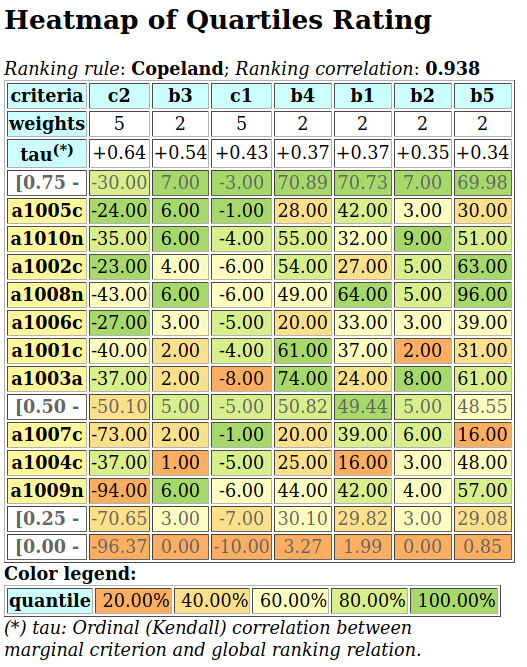
\includegraphics[width=7cm]{Figures/10-2-heatMap1.png}
\caption[Heatmap of absolute quartiles ranking]{\emph{Heatmap of absolute quartiles ranking}. The quartile equivalence classes appear lower-closed. No alternative is rated into the \texttt{Q1} class ($[0.00 - 0.25[$) and no alternative is rated into the Q4 class ($[0.75 - 1.00]$)}
\label{fig:10.2}       % Give a unique label
\end{figure}
	    
Using furthermore a specialised version of the \texttt{exportGraphViz()} method allows drawing in Figure~\vref{fig:10.3} the same rating result in a Hasse diagram format.\footnote{Note that the graphviz dot file was post-edited in order to mark in blue alternatives \texttt{a1001} and \texttt{a1010}.}
\begin{lstlisting}
>>> lqr.exportRatingGraphViz('quartileRatingDigraph')
 *---- exporting a dot file for GraphViz tools ---------*
  Exporting to quartileRatingDigraph.dot
  dot -Grankdir=TB -Tpng quartileRatingDigraph.dot -o quartileRatingDigraph.png
\end{lstlisting}
\begin{figure}[ht]
%\sidecaption[t]
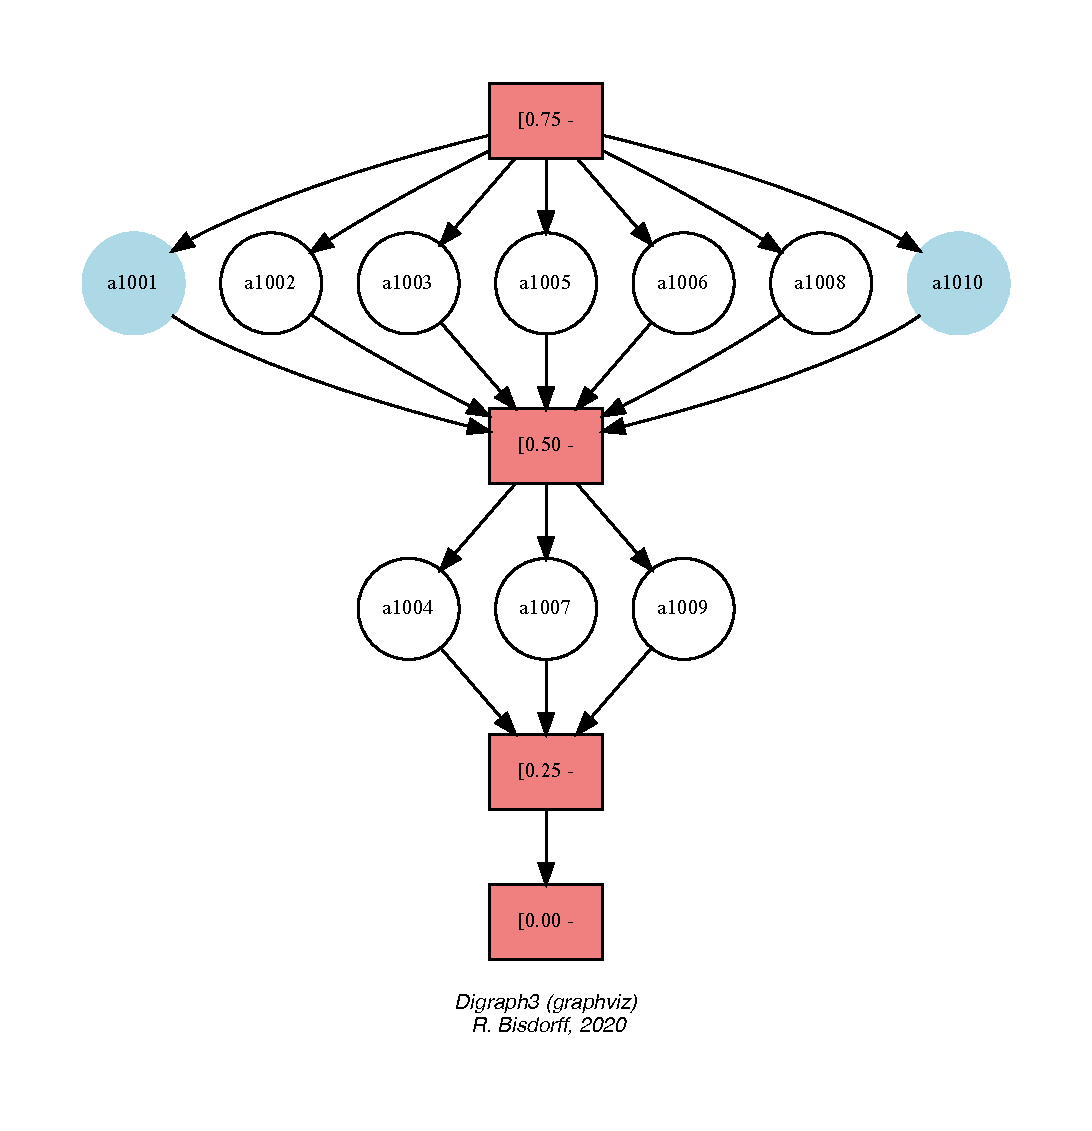
\includegraphics[width=\hsize]{Figures/10-3-normedRatingDigraph.pdf}
\caption{Absolute quartiles rating digraph}
\label{fig:10.3}       % Give a unique label
\end{figure}

We have actually solved now the \emph{absolute rating} problem stated at the beginning. Decision alternatives \texttt{a1001} and \texttt{a1010} (see Tab.~\vref{tab:10.1}) are both rated into the same third quartile \texttt{Q3} class (see Fig.~\vref{fig:10.3}), even if the \Copeland ranking, obtained from the underlying strict outranking digraph (see Fig.~\vref{fig:10.2}), suggests that alternative \texttt{a1010} is effectively \emph{better performing than} alternative \texttt{a1001}. 

A \emph{preciser} rating result may indeed be achieved when using \emph{deciles} instead of \emph{quartiles} for estimating the historical marginal cumulative distribution functions.
\begin{lstlisting}[caption={Absolute deciles rating result},label=list:10.9]
>>> pq1 = PerformanceQuantiles(pt, numberOfBins = 'deciles',\
...                 LowerClosed=True)
>>> pq1.updateQuantiles(newTab,historySize=None)
>>> lqr1 = LearnedQuantilesRatingDigraph(pq1,newActions,rankingRule='best')
>>> lqr1.showQuantilesRating()
  *-------- Deciles rating result ---------
   [0.60 - 0.70[ ['a1005', 'a1010', 'a1008', 'a1002']
   [0.50 - 0.60[ ['a1006', 'a1001', 'a1003']
   [0.40 - 0.50[ ['a1007', 'a1004']
   [0.30 - 0.40[ ['a1009']
\end{lstlisting}

Compared with the quartiles rating result, we notice in Listing~\vref{list:10.9} that the seven alternatives (\texttt{a1001}, \texttt{a1002}, \texttt{a1003}, \texttt{a1005}, \texttt{a1006}, \texttt{a1008} and \texttt{a1010}), rated before into the third quartile class $[0.50-0.75[$, are now divided up: alternatives \texttt{a1002}, \texttt{a1005}, \texttt{a1008} and \texttt{a1010} attain now the 7th decile class $[0.60-0.70[$, whereas alternatives \texttt{a1001}, \texttt{a1003} and \texttt{a1006} attain only the 6th decile class $[0.50-0.60[$. Of the three \texttt{Q2} $[0.25-0.50[$ rated alternatives (\texttt{a1004}, \texttt{a1007} and \texttt{a1009}), alternatives \texttt{a1004} and \texttt{a1007} are now rated into the 5th decile class $[0.40-0.50[$ and \texttt{a1009} is lowest rated into the 4th decile class $[0.30-0.40[$.

A browser heatmap view in Figure~\vref{fig:10.4} more conveniently illustrates this refined rating result.
\begin{lstlisting}
>>> lqr1.showHTMLRatingHeatmap(\
...       pageTitle='Heatmap of the deciles rating',\
...       colorLevels=5, Correlations=True)
\end{lstlisting}
\begin{figure}[ht]
\sidecaption[t]
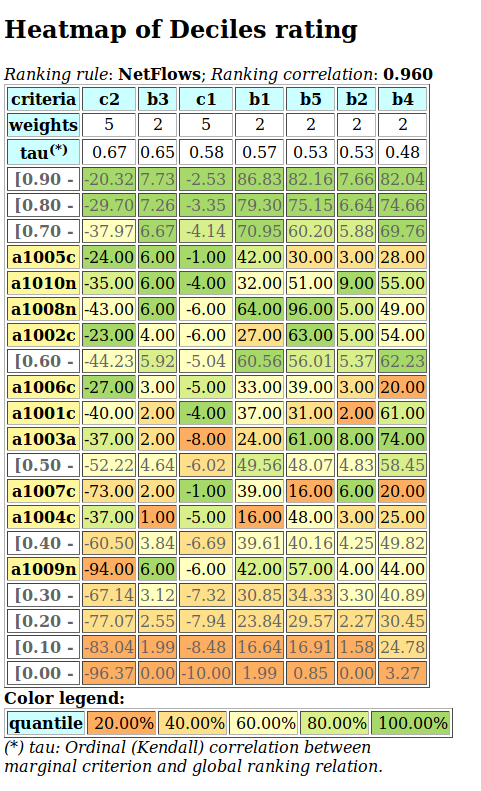
\includegraphics[width=7cm]{Figures/10-4-heatMap2.png}
\caption[Heatmap of absolute deciles rating]{\emph{Heatmap of absolute deciles rating}. Decision alternatives \texttt{a1001} and \texttt{a1010} are now, as expected, rated in the $6^{th}$ decile (\texttt{D6}), respectively in the $7^{th}$ decile (\texttt{D7})}
\label{fig:10.4}       % Give a unique label
\end{figure}

To avoid having to recompute performance deciles from historical data when wishing to refine a rating result, it is useful, depending on the actual size of the historical data, to initially compute performance quantiles with a relatively high number of bins, for instance \emph{dodeciles} or even \emph{centiles}. It is then possible to interpolate on the fly \emph{quartiles} or \emph{deciles} for instance, when constructing the rating digraph. 
\begin{lstlisting}[caption={From deciles interpolated quartiles rating result},label=list:10.10]
>>> lqr2 = LearnedQuantilesRatingDigraph(pq1,newActions,
...                   quantiles='quartiles')
>>> lqr2.showQuantilesRating()
  *-------- Deciles rating result ---------
   [0.50 - 0.75[ ['a1005', 'a1010', 'a1002', 'a1008',
                  'a1006', 'a1001', 'a1003']
   [0.25 - 0.50[ ['a1004', 'a1007', 'a1009']
\end{lstlisting}

With the \texttt{quantiles} parameter (see List.~\vref{list:10.10} Line 2), we recover by interpolation the same quartiles rating as obtained directly with historical performance quartiles (see List.~\vref{list:10.8}). Mind that a correct interpolation of quantiles from a given cumulative distribution function requires more or less uniform distributions of observations in each bin. 
More generally, in the case of industrial production monitoring problems, for instance, where large volumes of historical performance data may be available, it can be of interest to estimate even more precisely the marginal cumulative distribution functions, especially when \emph{tail} rating results, i.e. distinguishing \emph{very best}, or \emph{very weak} multiple-criteria performances, become a critical issue. Similarly, the \texttt{historySize} parameter may be used for monitoring on the fly \emph{unstable} random multiple-criteria performance data \citep{CHAM-2006}.  	

%%%%%%%
%The chapter bibliography
%\normallatexbib
%\clearpage
%\phantomsection
%\addcontentsline{toc}{section}{References}
%\input{02-mainMatters/10-chapterAbsoluteRating.bbl} 
\bibliographystyle{spbasic}
\bibliography{03-backMatters/reference}
 
\bibliographystyle{spbasic}
\bibliography{03-backMatters/reference}
 
\bibliographystyle{spbasic}
\bibliography{03-backMatters/reference}
 
